\documentclass[11pt]{article}

\usepackage[T1]{fontenc}
\usepackage{lmodern}
\usepackage{microtype}
\usepackage[margin=1in]{geometry}
\usepackage{xcolor}
\usepackage{booktabs}
\usepackage{tabularx}
\usepackage{longtable}
\usepackage{enumitem}
\usepackage{listings}
\usepackage{graphicx}
\usepackage{placeins}
\usepackage{etoolbox}
\usepackage{hyperref}

% Flush pending floats at every subsection boundary so a figure cannot drift out
% of the step that introduces it and land in the middle of a later step's
% listing.  Hooked after hyperref, which redefines the sectioning commands.
\pretocmd{\subsection}{\FloatBarrier}{}{}

\graphicspath{ {../common/figures/} }

\hypersetup{
  colorlinks=true,
  linkcolor=blue!60!black,
  urlcolor=blue!60!black
}

\lstdefinestyle{minrv}{
  basicstyle=\ttfamily\small,
  columns=fullflexible,
  keepspaces=true,
  showstringspaces=false,
  frame=single,
  rulecolor=\color{black!15},
  breaklines=true
}

\lstdefinelanguage{tcl}{
  morekeywords={set,foreach,if,file,exists,glob,set_property,get_files,get_filesets,current_fileset,join,lindex},
  sensitive=true,
  morecomment=[l]{\#},
  morestring=[b]"
}

\newcommand{\ProjectName}{MinRV32}

\title{\ProjectName: A Hands-On, Open-Source RV32I Pipeline for Teaching Digital Design from RTL to FPGA}
\author{Project documentation (compiled from \texttt{docs/})}
\date{\today}

\begin{document}
\sloppy
\maketitle

\begin{abstract}
\ProjectName\ is an educational RV32I processor implemented as a clean, modular,
five-stage pipeline (F/D/E/M/W) in VHDL. The design is intentionally small but
complete: it includes forwarding, stall/flush hazard handling, a Harvard
instruction/data memory split, a linker-aware memory map, and a practical build
flow that uses a RISC-V GCC toolchain to generate hex images for IMEM/DMEM.
This document consolidates the repository documentation into a single,
coursework-friendly overview and quickstart.
\end{abstract}

\tableofcontents
\newpage

\section{Project showcase: an educational route from RTL to FPGA}

This section presents the project as a sequence of short, reproducible labs.
Each step produces something you can inspect: waveforms, traces, signatures, or
on-board memory state. Figure~\ref{fig:route-overview} gives the overall route
from editing the RTL to validating on the FPGA.

\begin{figure}[ht]
  \centering
  \fbox{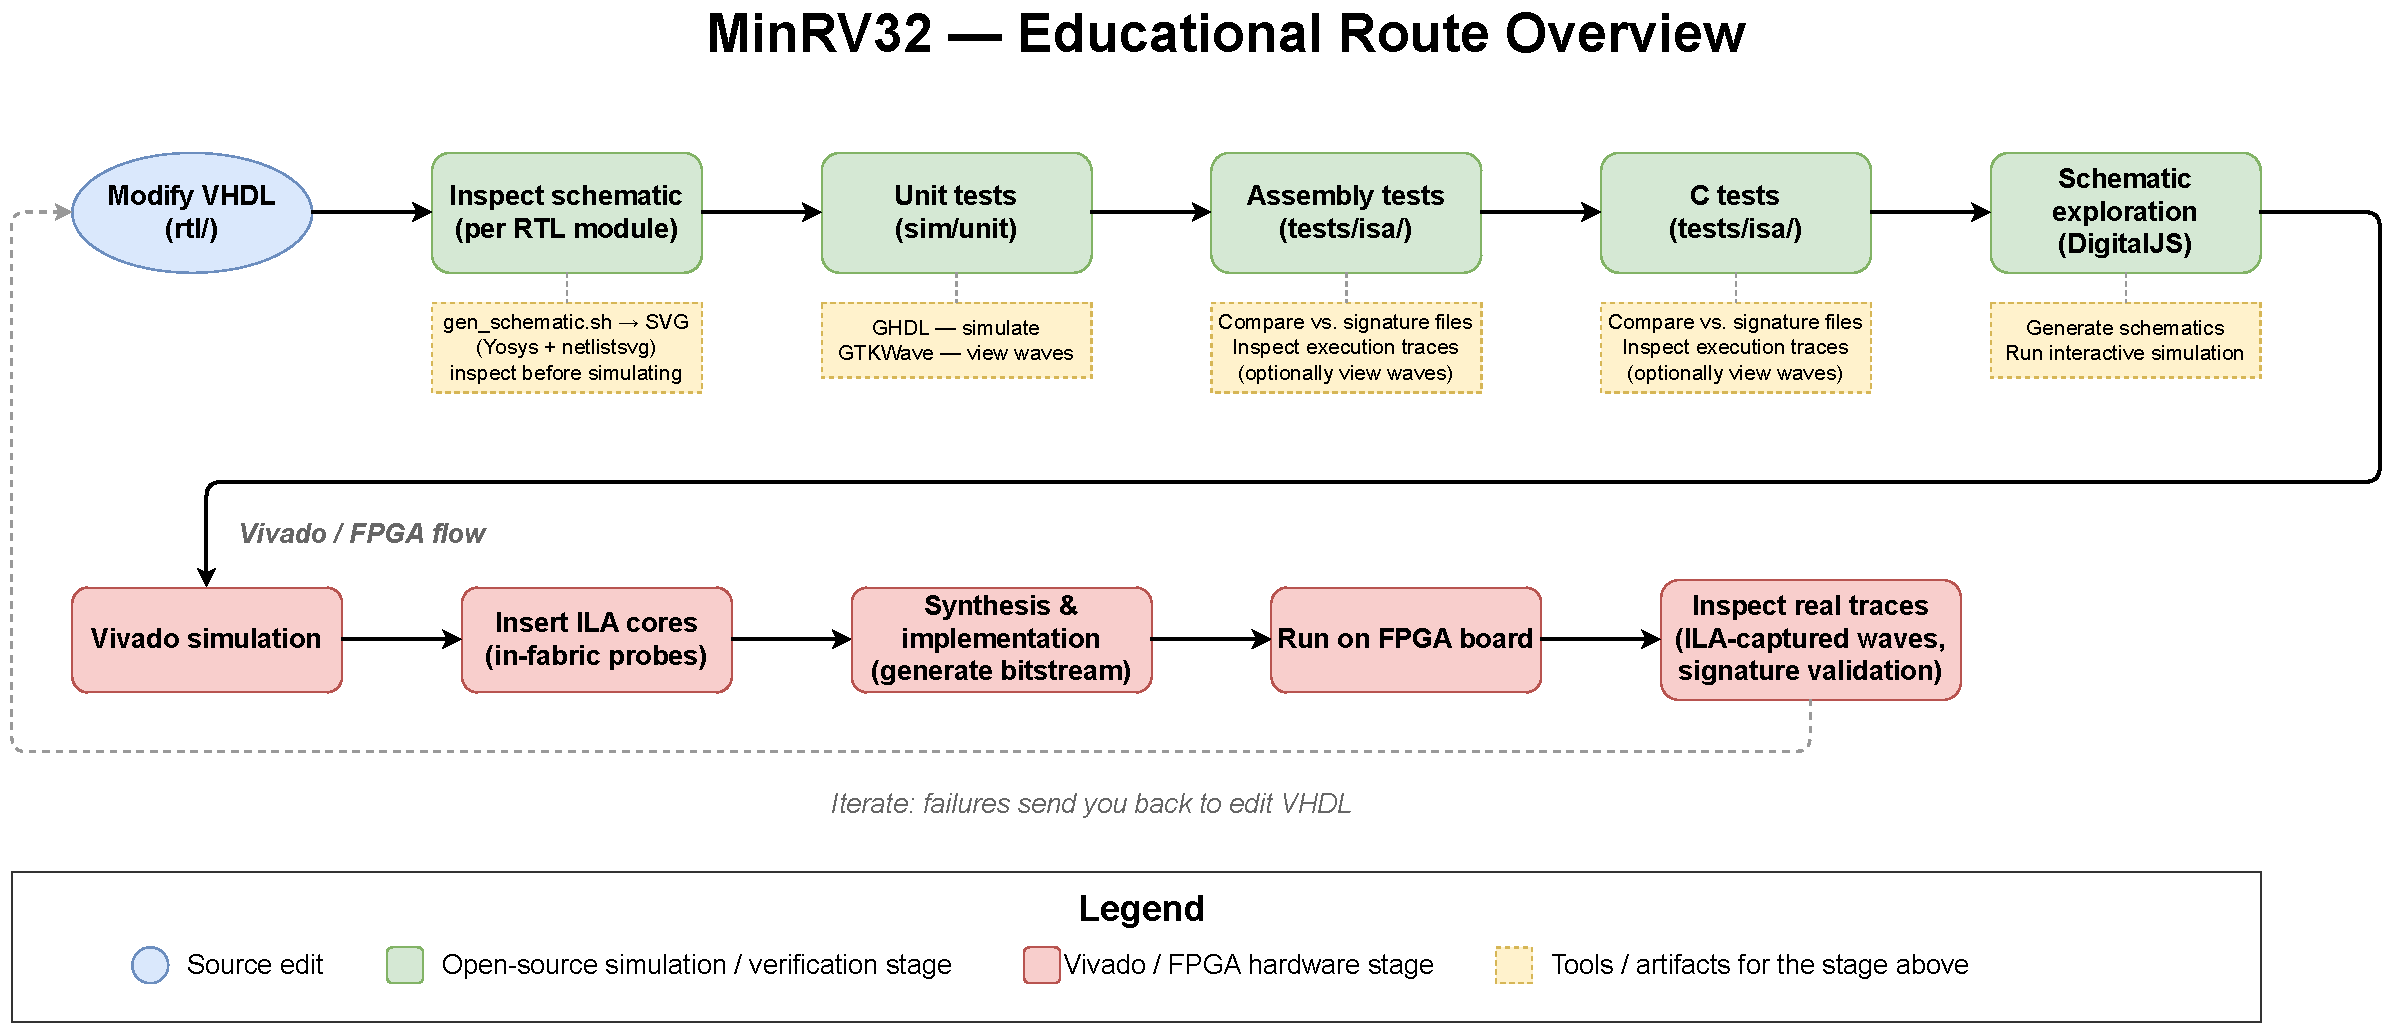
\includegraphics[width=0.97\linewidth]{educational_workflow.pdf}}
  \caption{Educational route overview. After editing the RTL, a module's
  schematic can be generated for inspection (Yosys + \texttt{netlistsvg}) before
  any simulation is run. After simulation, the design can be implemented and validated on the FPGA with an ILA capture.}
  \label{fig:route-overview}
\end{figure}

\subsection{Step 1: read/modify VHDL}

The RTL is modular (ALU, regfile, hazard unit, memory access helper, etc.), so a
change is usually localized to one small, readable entity.

\paragraph{Example VHDL: ALU combinational process (complete \texttt{case} statement)}
\lstinputlisting[style=minrv,language=VHDL,firstline=51,lastline=98]{../../rtl/alu.vhd}

\subsection{Step 2: inspect a module's schematic (before simulating)}

Before running any simulation, the structure of an edited module can be checked
visually. \texttt{scripts/gen\_schematic.sh} synthesizes an entity with Yosys
(via its GHDL front-end) and renders an SVG schematic with \texttt{netlistsvg},
so design mistakes are often caught just by looking at the elaborated logic.
\begin{lstlisting}[style=minrv]
./scripts/gen_schematic.sh --list           # list discoverable RTL entities
./scripts/gen_schematic.sh alu              # hierarchical schematic of one module
./scripts/gen_schematic.sh --flat 1 riscvpipe  # expand one level of hierarchy
\end{lstlisting}
The SVG lands under \texttt{build/schematics/<entity>.svg}
(Figure~\ref{fig:schematic-alu} shows the result for the \texttt{alu} entity).
The same tool underlies the microarchitecture block diagrams in this manual and
the DigitalJS export described in Step~6 (Section~\ref{sec:digitaljs}); see that
section for the prerequisite packages.

\begin{figure}[ht]
  \centering
  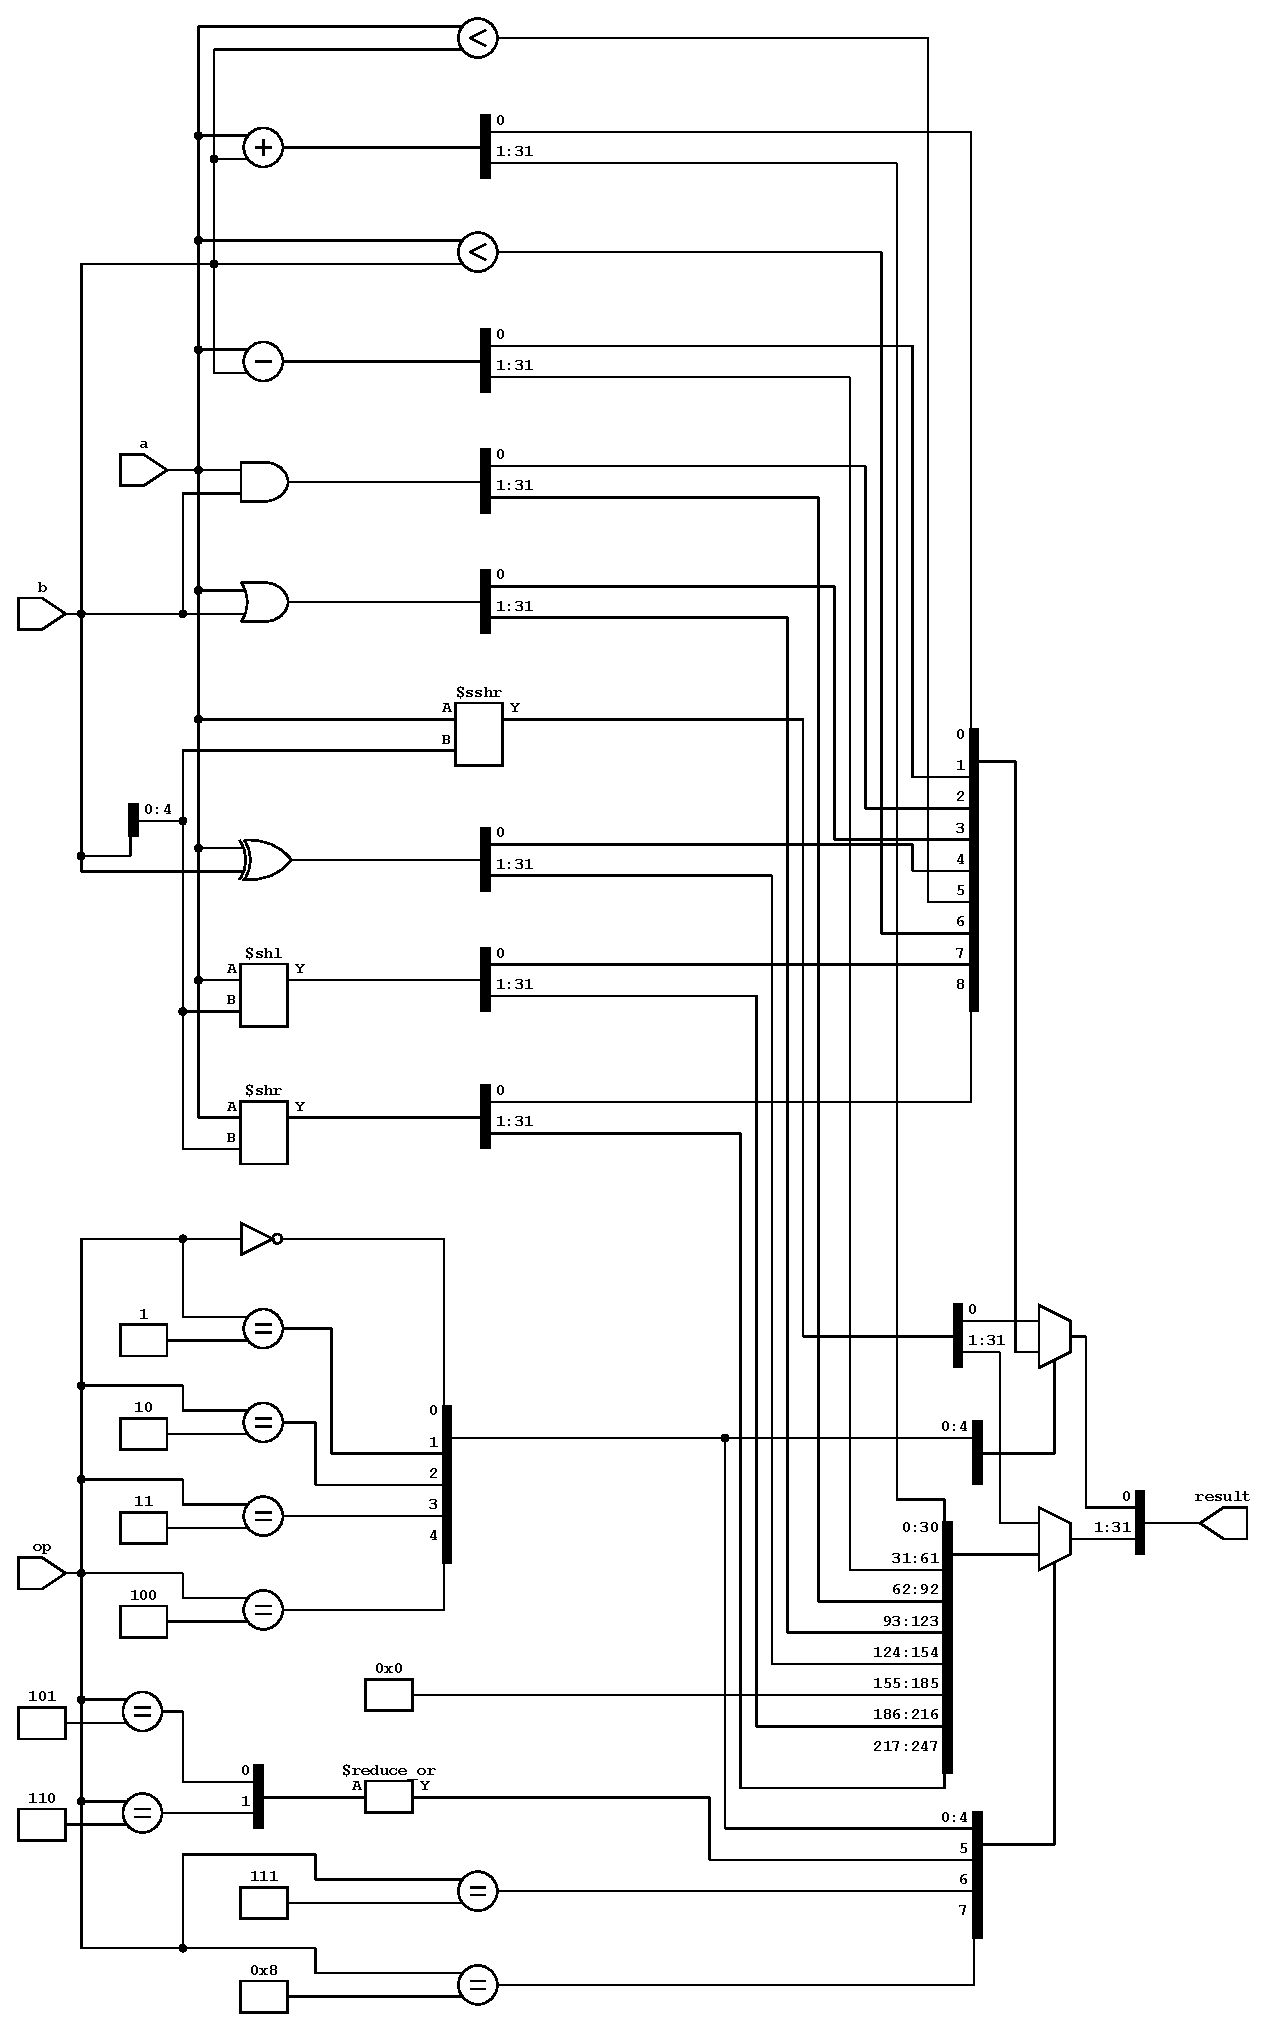
\includegraphics[height=0.82\textheight,keepaspectratio]{alu.pdf}
  \caption{Elaborated schematic of the \texttt{alu} entity rendered by
  \texttt{gen\_schematic.sh} (Yosys + \texttt{netlistsvg}). The \texttt{op}
  decoder (\texttt{\$eq} comparators, left of centre) selects, through the
  output multiplexers, one of the candidate results computed by the arithmetic,
  shift, and comparison operators. By default the script drops the
  multiplexers' don't-care default input for the unused \texttt{op} encodings
  (\texttt{opt\_expr -mux\_undef}), so no floating stubs clutter the diagram;
  pass \texttt{--keep-undef} to keep them.}
  \label{fig:schematic-alu}
\end{figure}

\subsection{Step 3: simulate modules with unit testbenches}

For component bring-up, the repository includes small self-checking unit
testbenches under \texttt{sim/unit/}.

\paragraph{Example unit testbench: checking the ALU (complete architecture body)}
\lstinputlisting[style=minrv,language=VHDL,firstline=89,lastline=116]{../../sim/unit/tb_alu.vhd}

\paragraph{Run + dump waves}
\begin{lstlisting}[style=minrv]
./scripts/run_unit_tb.sh --fst alu
./scripts/view_wave.sh build/waves/tb_alu.fst
\end{lstlisting}
GTKWave then shows the unit-test waveform (Figure~\ref{fig:wave-tb-alu}).

\begin{figure}[ht]
  \centering
  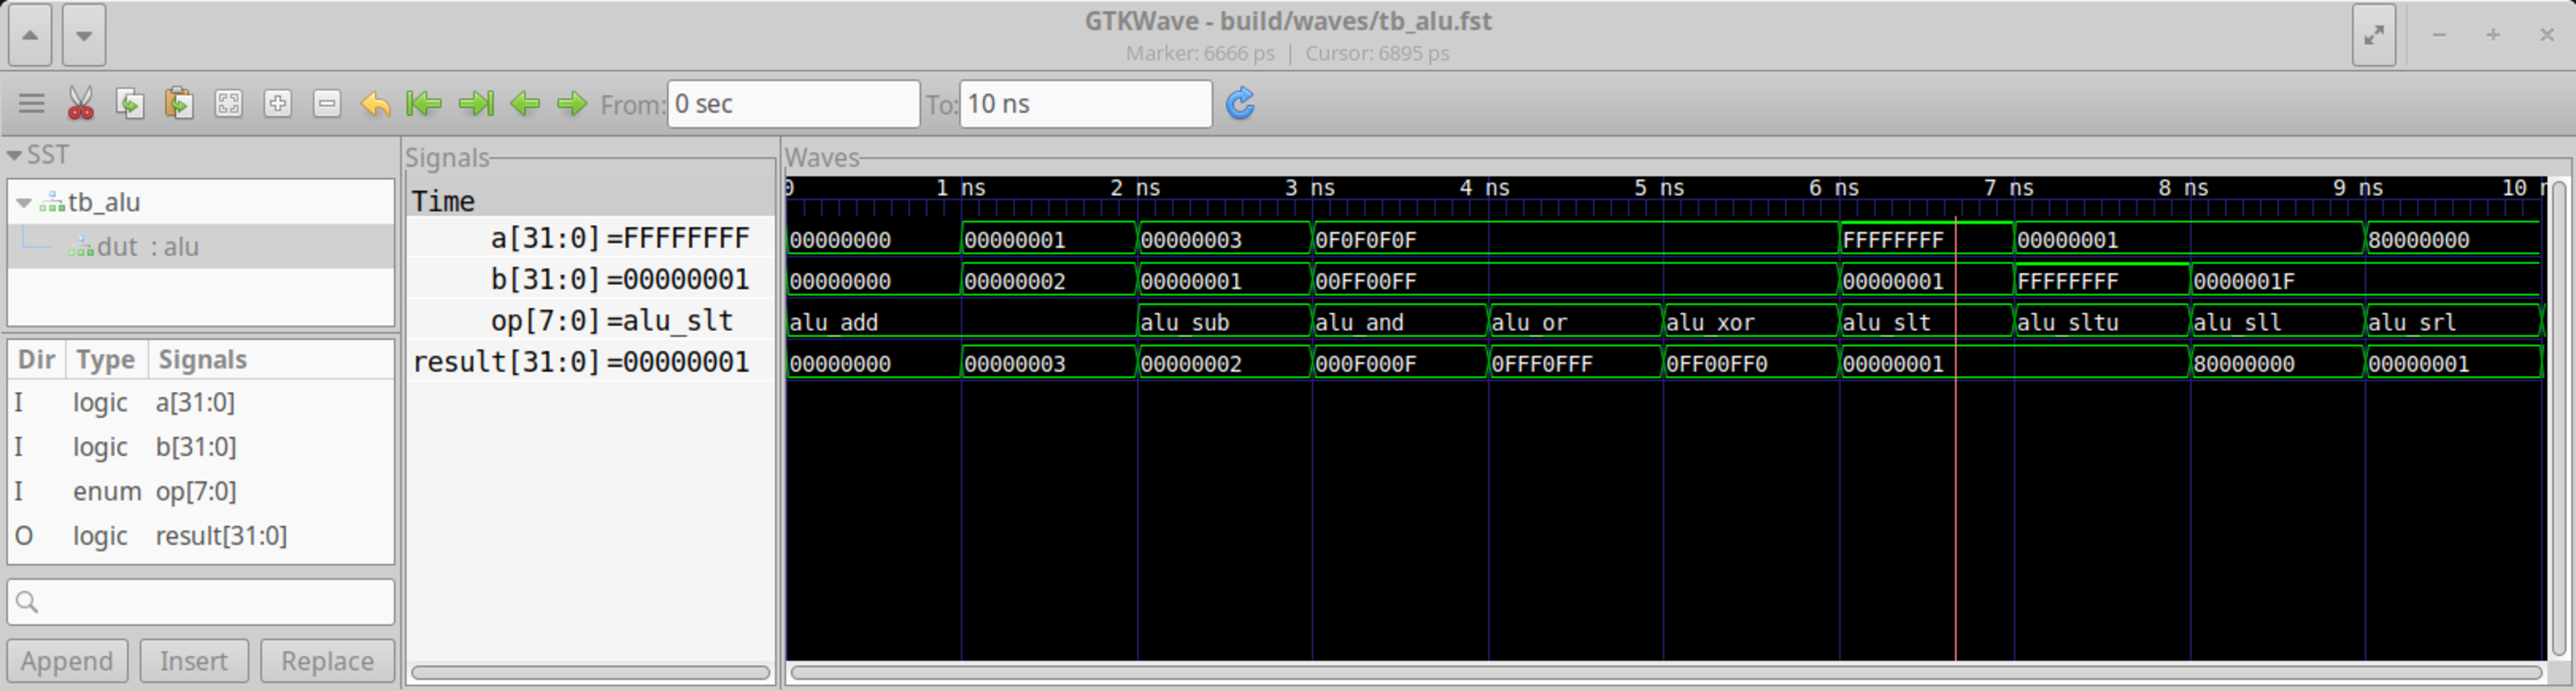
\includegraphics[scale=0.29]{gtkwave-tb_alu.pdf}
  \caption{Unit-test waveform.}
  \label{fig:wave-tb-alu}
\end{figure}

\subsection{Step 4: run assembly tests (correctness via signature + optional traces/waves)}

Integration tests live under \texttt{tests/isa/}. Each test writes a signature
window into DMEM at \texttt{0x20000100}. The expected values are stored in
\texttt{tests/isa/<name>.sig}, and the testbench compares observed vs expected.

\paragraph{Example assembly test: write 6 signature words}
\lstinputlisting[style=minrv,firstline=1,lastline=32]{../../tests/isa/addi_only.S}

\paragraph{Run + view trace and waves}
\begin{lstlisting}[style=minrv]
./scripts/run_test.sh --trace addi_only
./scripts/run_test.sh --fst addi_only
./scripts/view_wave.sh build/waves/addi_only.fst
\end{lstlisting}

\paragraph{Per-instruction trace: decoded ASM + stage control sample output}
\lstinputlisting[style=minrv,firstline=22,lastline=49]{../common/sample_output/addi_only_trace.txt}

\subsection{Step 5: run freestanding C tests (same signature mechanism)}

Freestanding C tests follow the same rule: compute deterministic values, then
store them into the signature window at \texttt{0x20000100}.

\paragraph{Example C: tests/isa/factorial.c}
\lstinputlisting[style=minrv,language=C,firstline=1,lastline=31]{../../tests/isa/factorial.c}

\paragraph{Run + view trace and waves}
\begin{lstlisting}[style=minrv]
./scripts/run_test.sh --trace factorial
./scripts/run_test.sh --fst factorial
./scripts/view_wave.sh build/waves/factorial.fst
\end{lstlisting}

\paragraph{Example test output snippet without trace}
\lstinputlisting[style=minrv,firstline=9,lastline=20]{../common/sample_output/factorial.txt}

The resulting execution waveform for computing $6!$ is shown in
Figure~\ref{fig:wave-factorial}.

\begin{figure}[ht]
  \centering
  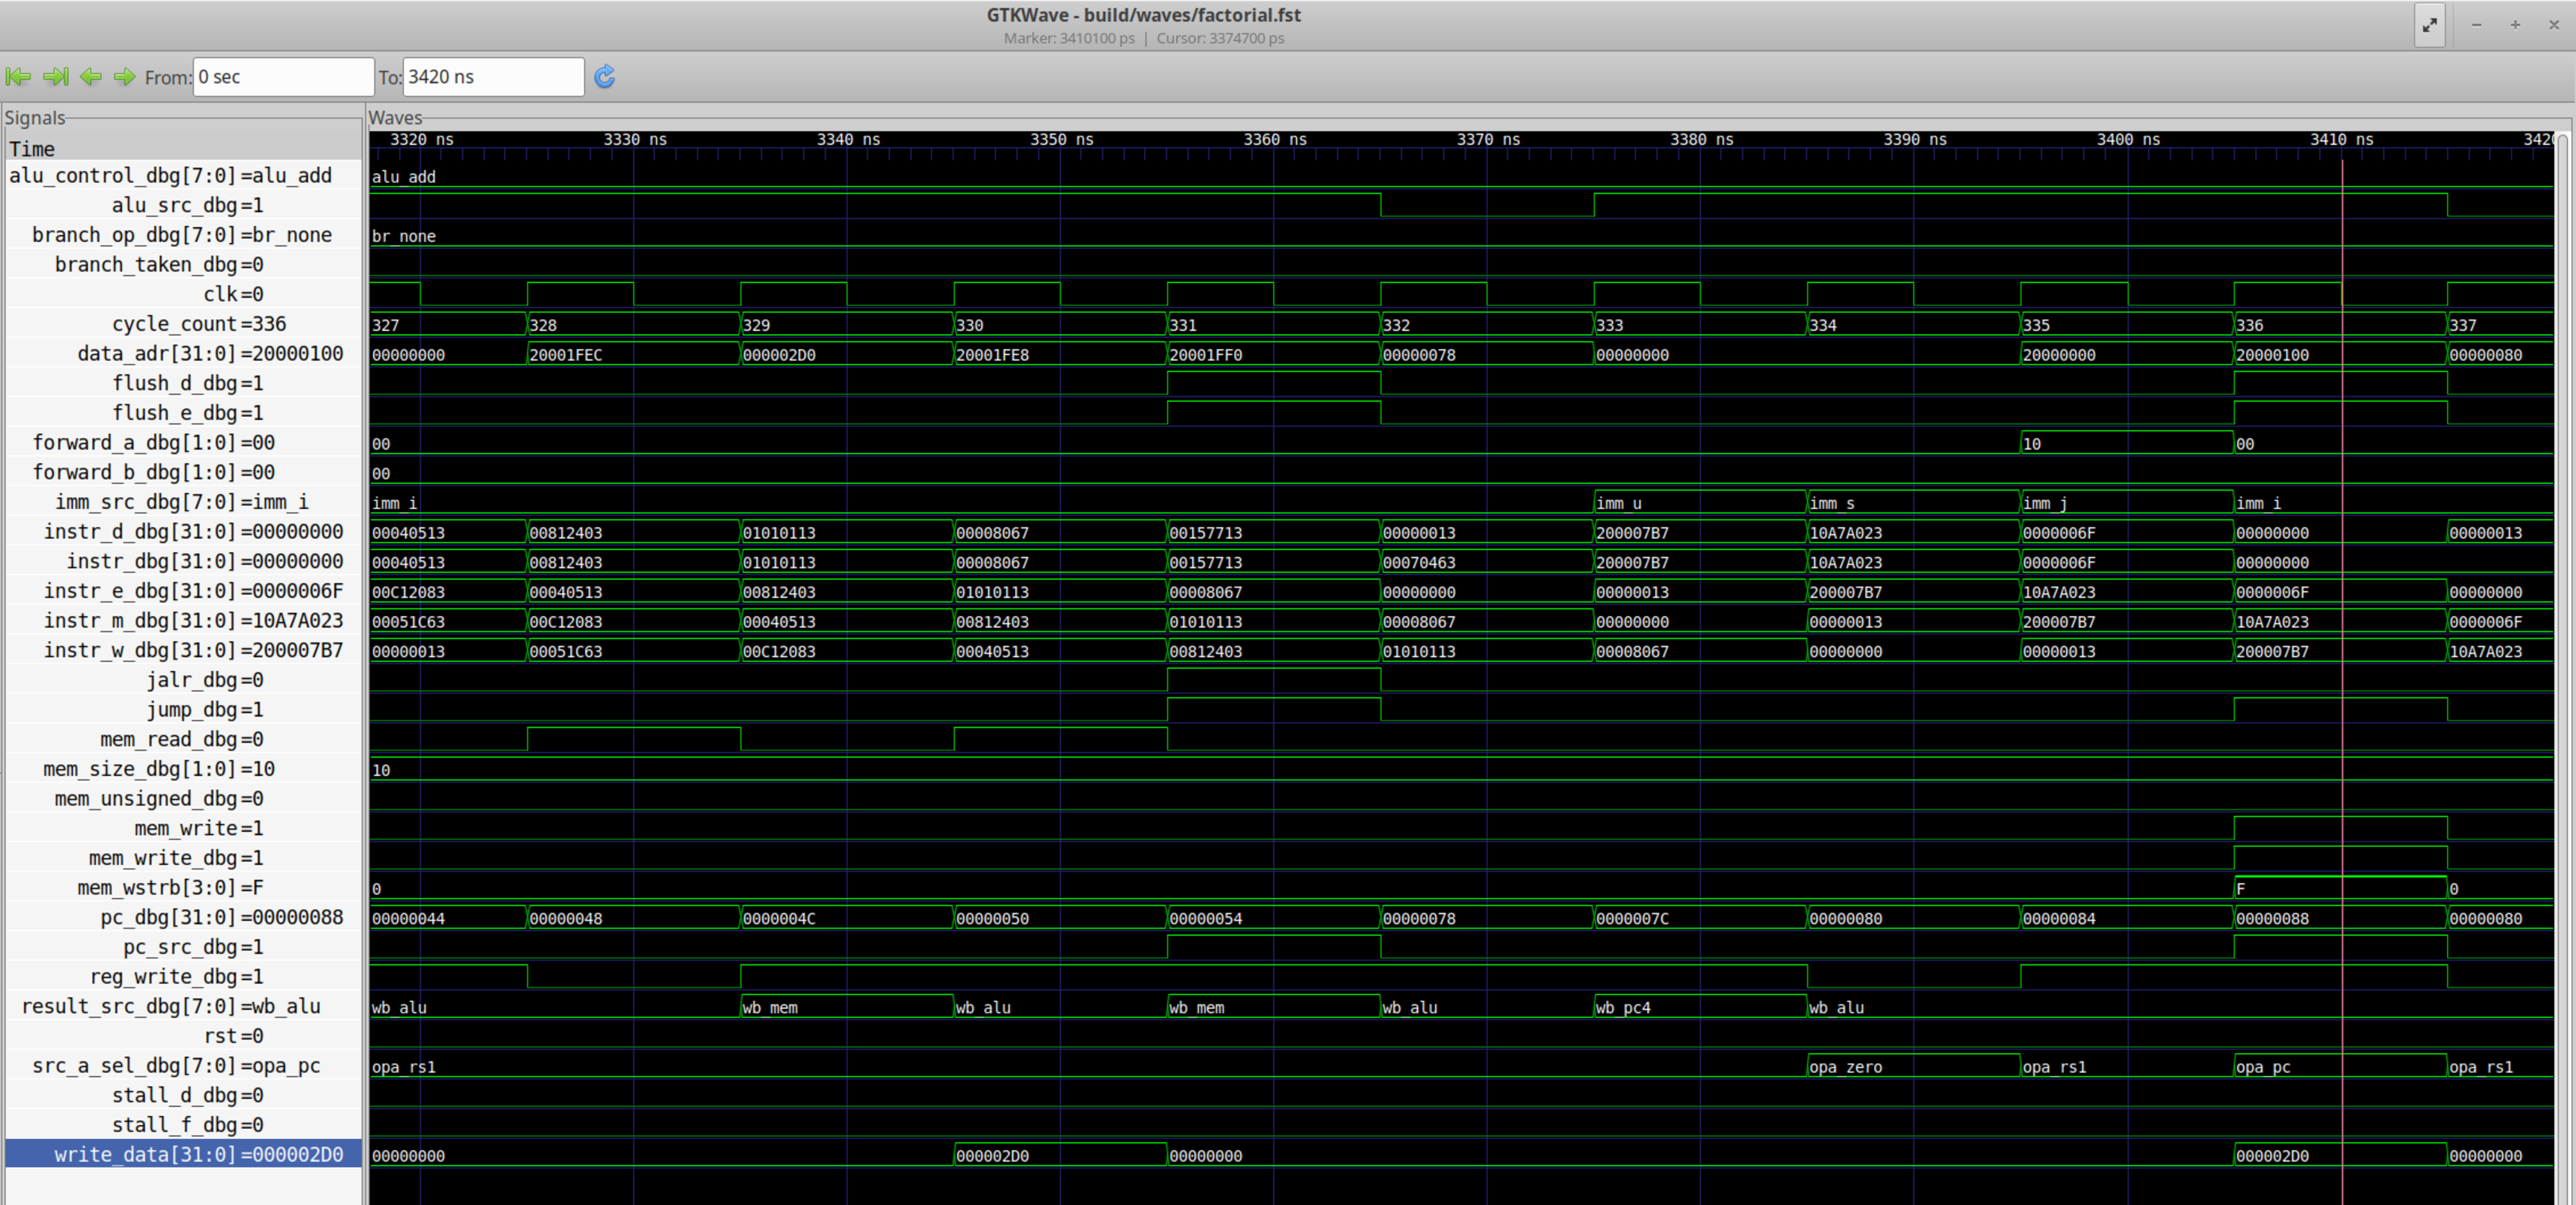
\includegraphics[scale=0.2]{gtkwave-factorial.pdf}
  \caption{Factorial C program execution waveform for calculating 6!}
  \label{fig:wave-factorial}
\end{figure}

\subsection{Step 6: explore the design interactively in DigitalJS}

The same netlist that produces the static schematics of Step~2 can be exported
to DigitalJS for interactive, in-browser simulation: drive inputs by clicking
and watch values propagate through the gates. With real firmware pre-loaded it
even single-steps the whole pipeline. This is a visual complement to GTKWave
(for leaf modules) and to the full-core tests (for the whole pipeline); it is
not signature-checked, so it does not replace the testbench pass/fail. See
Section~\ref{sec:digitaljs} for the commands and the firmware-loaded export.
Although the simulation is not signature-checked, it is a powerful tool
for visually confirming the design's behaviour on the FPGA, where visibility
is limited to the ILA capture points. Additionally, the signature values written
in the DMEM, usually at the end of the executed program, can be manually
verified against the expected values in the corresponding \texttt{.sig} file. 

\subsection{Step 7: implement on FPGA and validate with an ILA capture}

After simulation passes, Vivado can synthesize and implement the same RTL. On
hardware, you validate results with an Integrated Logic Analyzer (ILA)
triggered on stores into the signature window -- the same \texttt{.sig} words
that simulation already checks (Figure~\ref{fig:ila-full_core}).

\paragraph{Content of the tests/isa/full\_core.sig file}
\lstinputlisting[style=minrv,firstline=1,lastline=10]{../../tests/isa/full_core.sig}

\begin{figure}[ht]
  \centering
  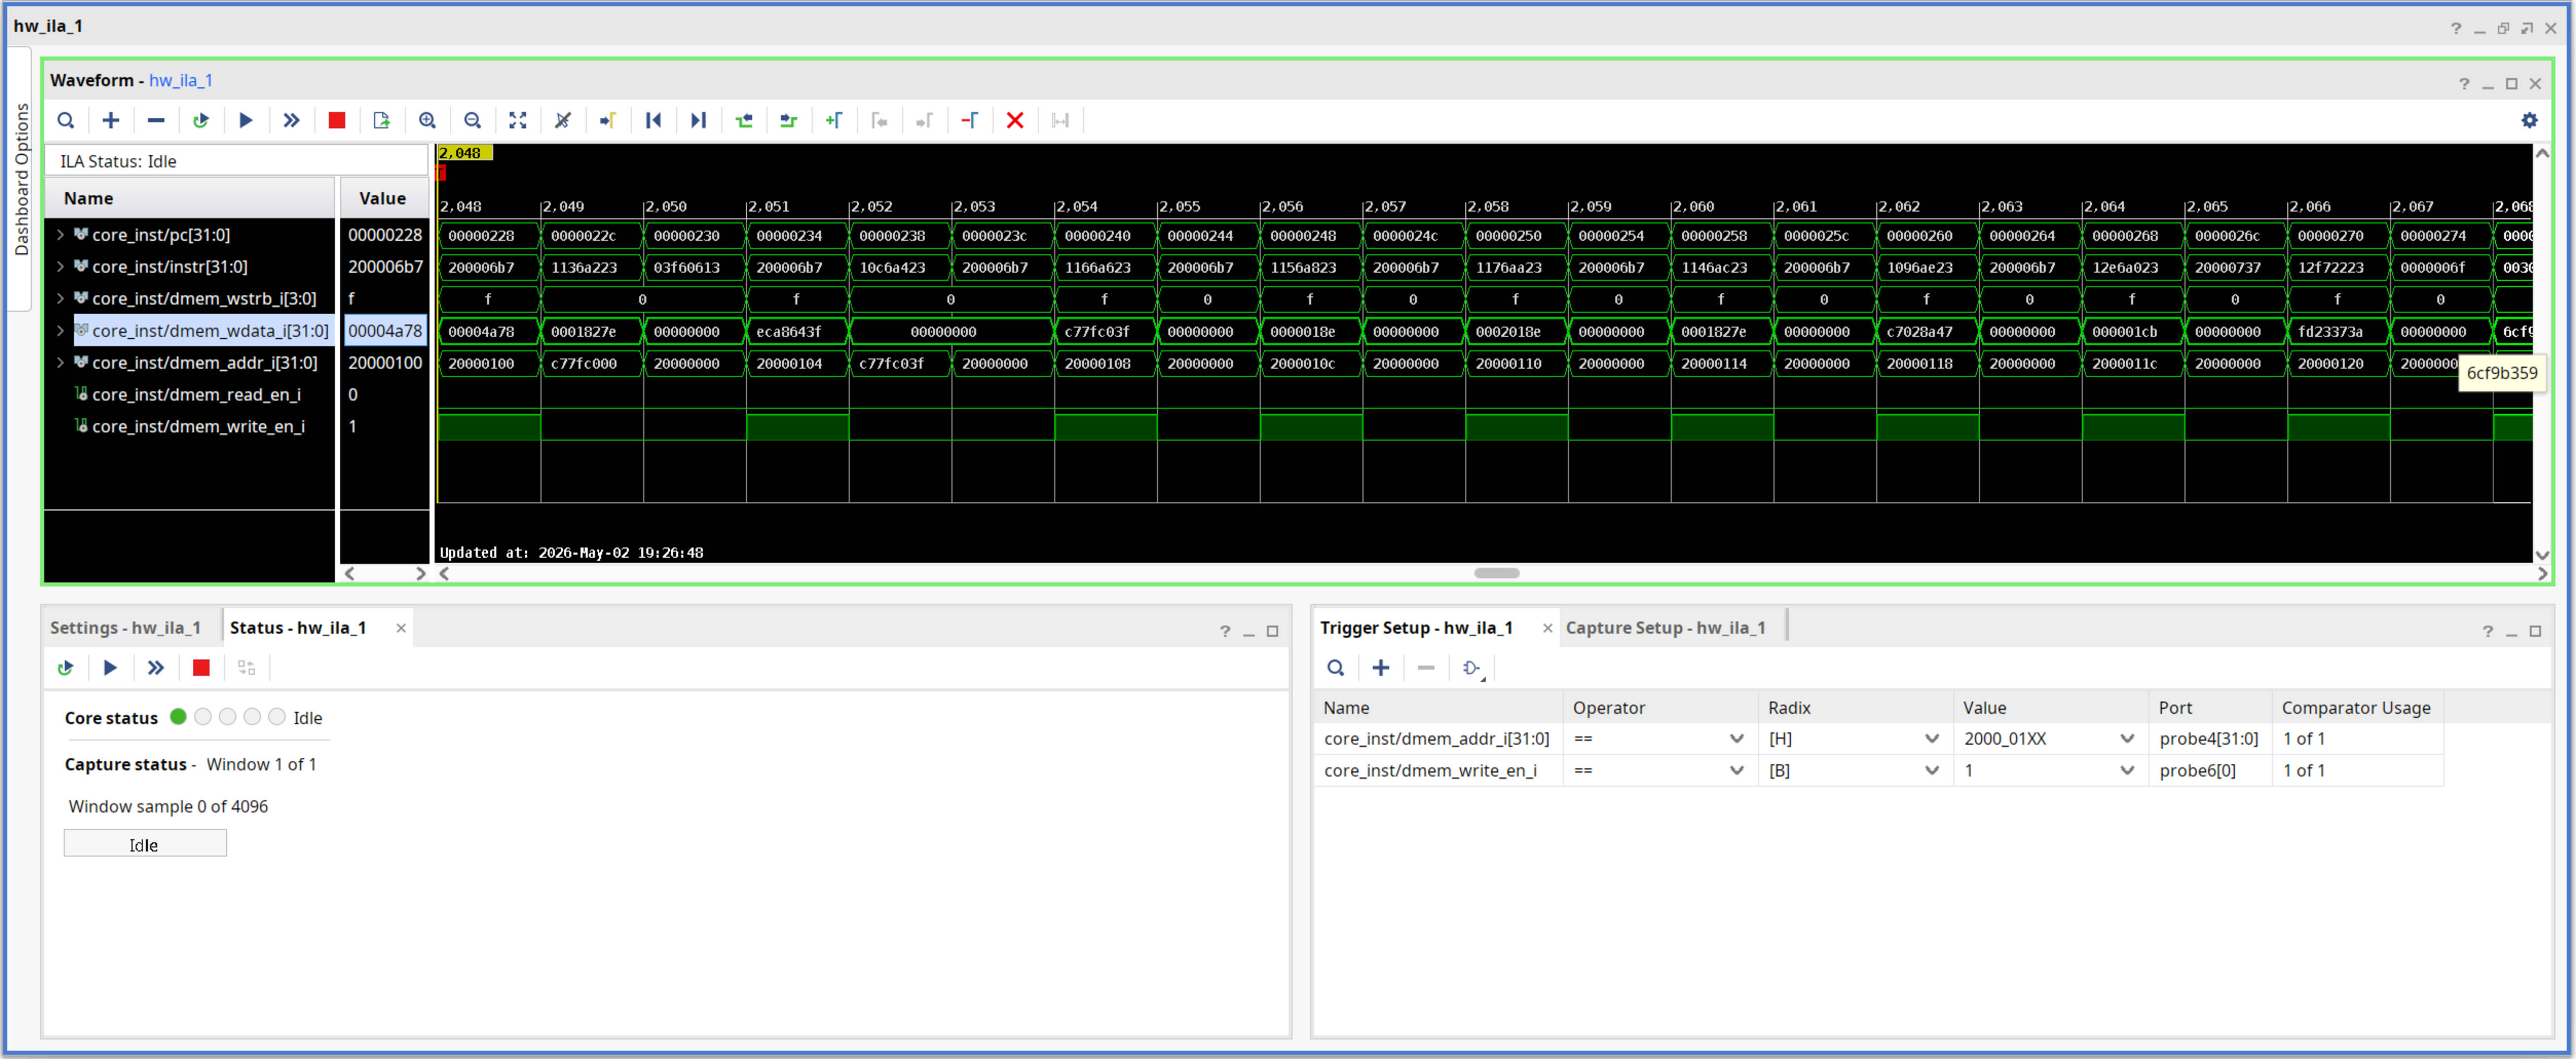
\includegraphics[scale=0.18]{ila-full_core.pdf}
  \caption{Hardware Manager + ILA waveform capturing signature stores of the full\_core.c program running on MinRV32 on the FPGA.}
  \label{fig:ila-full_core}
\end{figure}

\clearpage
\section{What this project is for}

\ProjectName\ is a teaching-oriented implementation of an RV32I pipelined CPU.
Its goal is to help you learn how a modern in-order pipeline is structured and
validated in an HDL, and how the resulting RTL maps onto FPGA-friendly building
blocks (especially synchronous Block RAMs).

\subsection{What you learn by studying or modifying this core}
\begin{itemize}[leftmargin=*]
  \item How a five-stage pipeline is partitioned (Fetch/Decode/Execute/Memory/Writeback) and how stage registers define timing.
  \item How a hazard unit combines forwarding, stalling, and flushing to preserve correctness.
  \item How a Harvard memory map and a custom linker script make bare-metal C programs \emph{actually runnable} on the hardware model.
  \item How to validate ISA behavior with directed tests and self-checking signatures.
  \item HDL coding practice: writing synthesizable RTL (design for synthesis) and writing testbenches for design verification.
  \item Using open-source tools to simulate, verify, and visualize HDL designs (e.g.\ GHDL, GTKWave, DigitalJS).
  \item How to simulate and debug in Xilinx Vivado (XSim), and how to instrument an FPGA build with ILA.
\end{itemize}

\subsection{Textbook lineage}
The RTL follows the structure and naming conventions of the Harris \& Harris
pipelined reference design (stage-suffixed signals such as \texttt{PCF},
\texttt{InstrD}, \texttt{ALUControlE}, \texttt{MemWriteM}, \texttt{ResultSrcW}).
Section~\ref{sec:textbook-deviations} summarizes the intentional deviations made
to support a synthesis-ready, BRAM-friendly implementation and a slightly richer
RV32I subset.


\clearpage
\section{Microarchitecture overview}

The core is a five-stage RV32I pipeline (F/D/E/M/W). Instructions overlap in
flight; stage boundaries are defined by pipeline registers, and a dedicated
hazard unit generates forwarding, stall, and flush control.
The block schematics in this section (Figures~\ref{fig:uarch-system}--\ref{fig:uarch-execute})
are generated directly from the RTL with Yosys and \texttt{netlistsvg} (via
\texttt{scripts/gen\_schematic.sh}) in hierarchical mode, so every labelled box
is a real sub-module instance. They progress from the system boundary
(Figure~\ref{fig:uarch-system}), through the core
(Figure~\ref{fig:uarch-core}) and the five datapath stages
(Figure~\ref{fig:uarch-stages}), down to one stage's internals
(Figure~\ref{fig:uarch-execute}).

\begin{figure}[t]
  \centering
  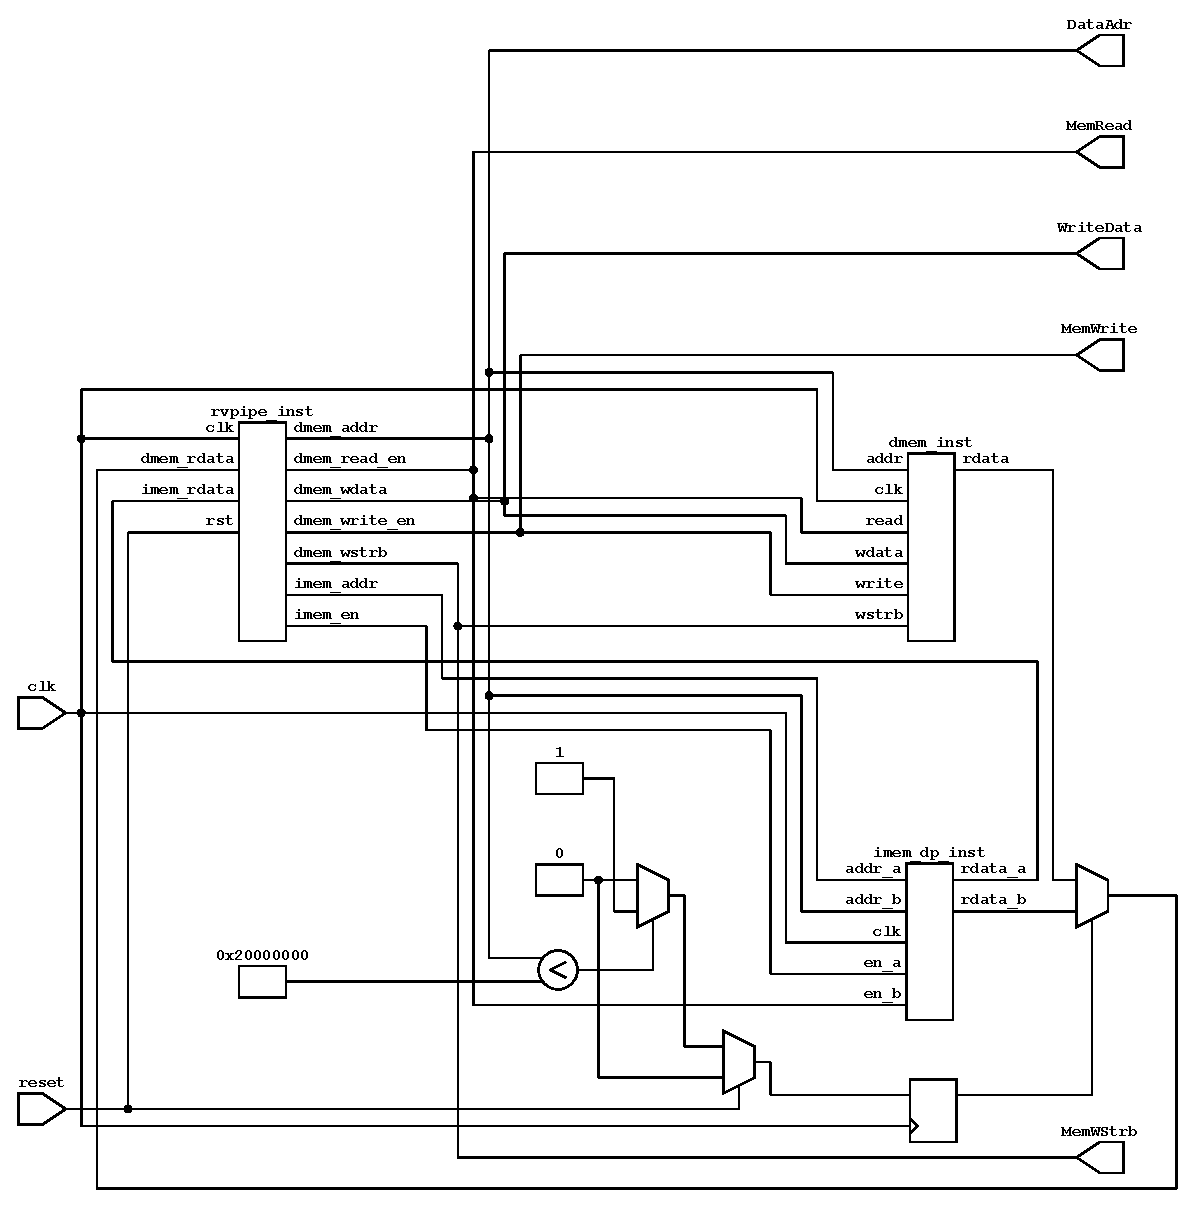
\includegraphics[width=0.62\linewidth]{uarch_system.pdf}
  \caption{System level (\texttt{top}). The synthesis top wires the pipelined
  core (\texttt{rvpipe\_inst}) to a dual-port instruction memory
  (\texttt{imem\_dp\_inst}) and a data memory (\texttt{dmem\_inst}); the dual-port
  IMEM also serves \texttt{.rodata} reads on port~B. Auto-generated with
  \texttt{netlistsvg}.}
  \label{fig:uarch-system}
\end{figure}

\begin{figure}[t]
  \centering
  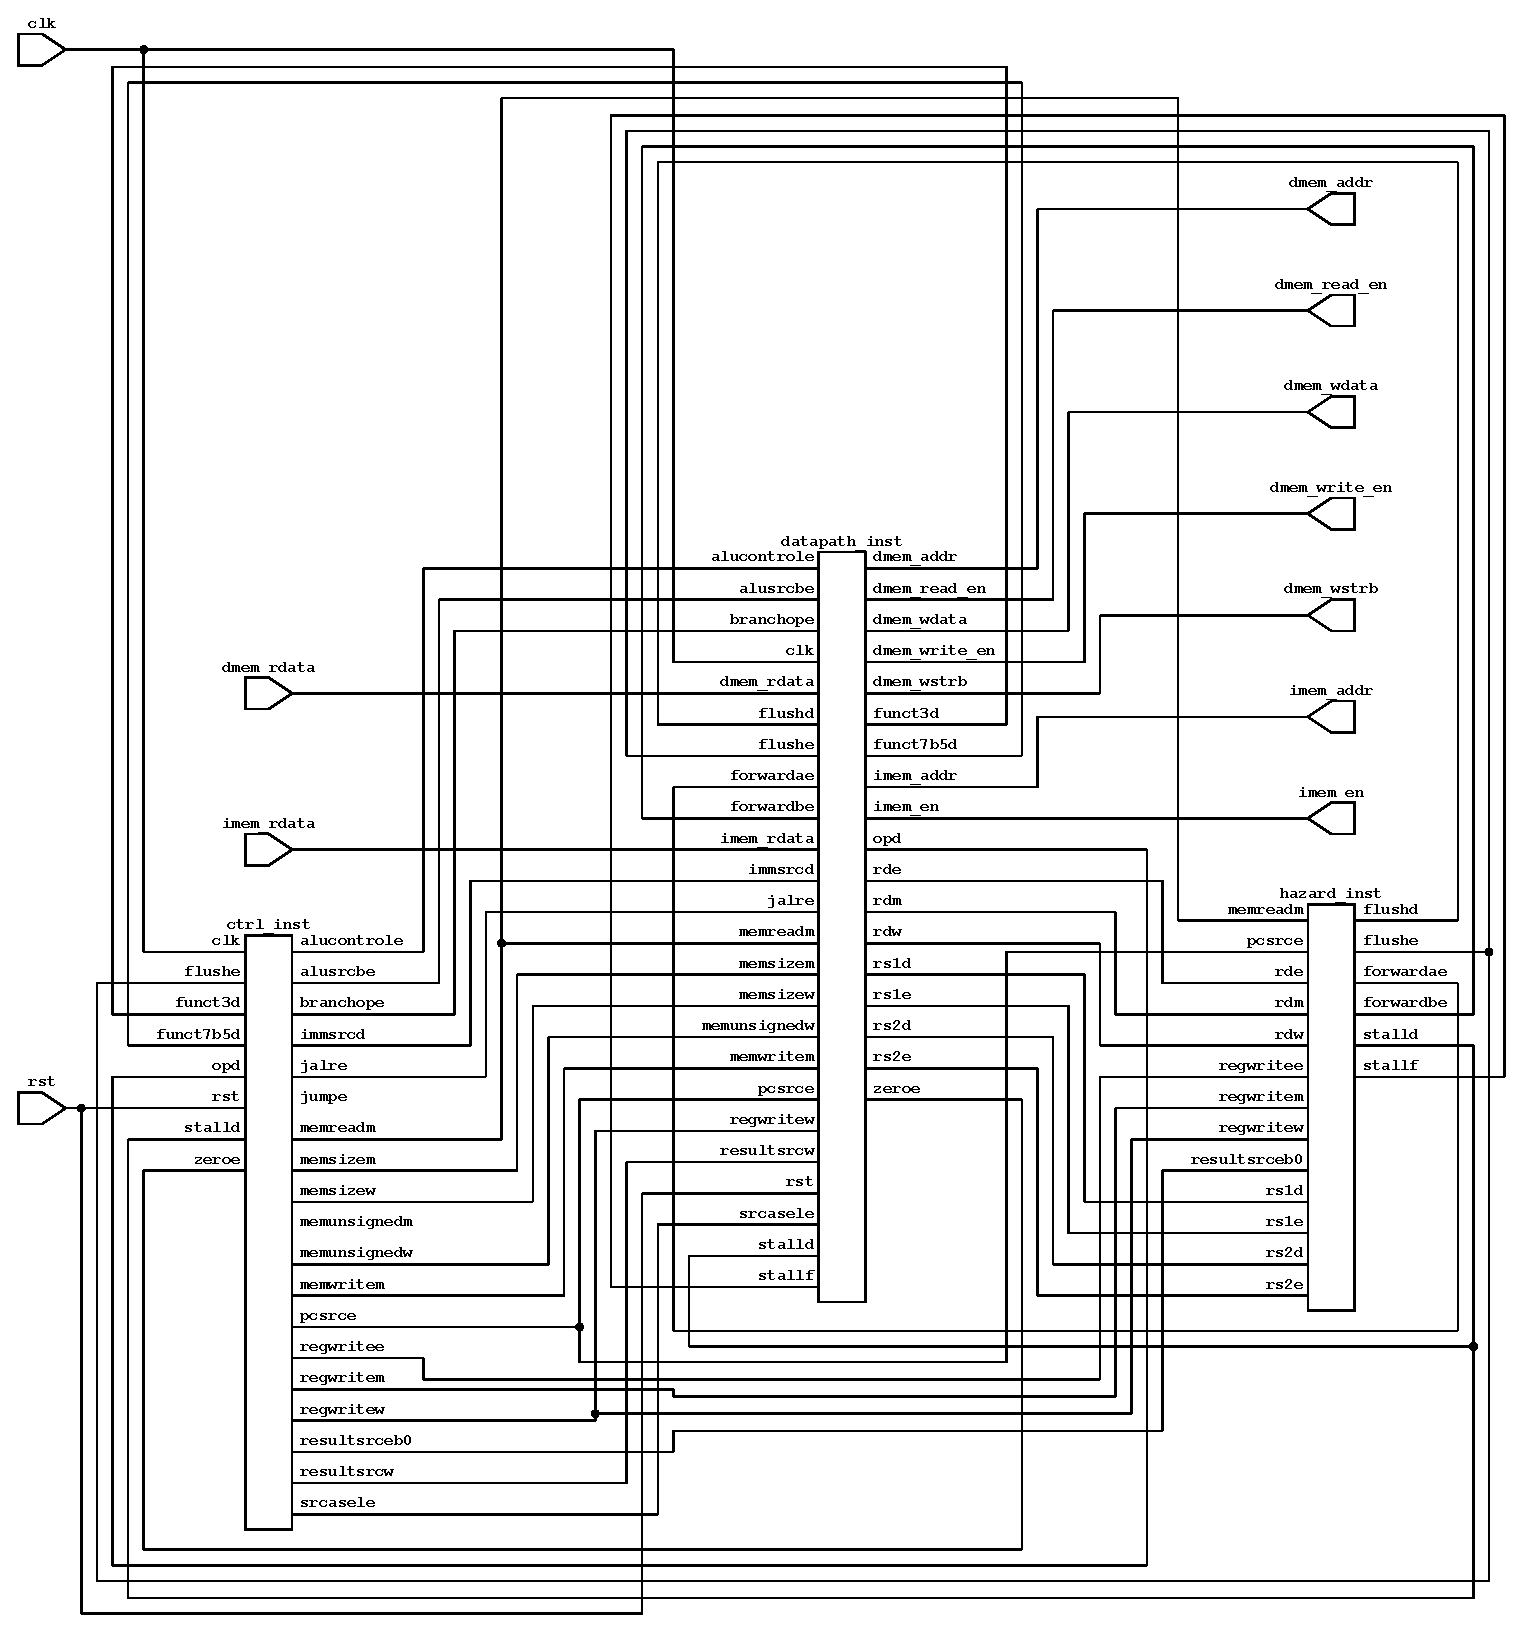
\includegraphics[width=\linewidth]{uarch_core.pdf}
  \caption{Core level (\texttt{riscvpipe}). The pipelined core binds the
  controller (\texttt{ctrl\_inst}), the structural datapath
  (\texttt{datapath\_inst}), and the hazard unit (\texttt{hazard\_inst}); the
  control and hazard nets between them are visible as the inter-block wiring.
  Auto-generated with \texttt{netlistsvg}.}
  \label{fig:uarch-core}
\end{figure}

\subsection{One detail that matters on FPGA: synchronous memories}
Instruction and data memories are written in a BRAM-friendly style with
synchronous reads. As a result, the registered memory outputs naturally align
with pipeline stage boundaries: the IMEM output provides \texttt{InstrD} and the
DMEM output provides \texttt{ReadDataW}. A small \texttt{flush\_d\_hold} mechanism
inserts a NOP after redirects to implement a textbook-style decode flush even
though BRAM outputs cannot be ``overwritten'' like a conventional F$\rightarrow$D
register.

\subsection{Stage-by-stage summary}
\begin{description}[leftmargin=*,labelwidth=2.2cm]
  \item[Fetch (F)] A \texttt{PCF} register feeds the instruction memory address.
  Next-PC selection chooses \texttt{PC+4} or an Execute-stage redirect
  (taken branch/jump or JALR).
  \item[Decode (D)] The controller decodes opcode/funct fields and the register
  file reads \texttt{rs1}/\texttt{rs2}. Immediate expansion produces
  \texttt{ImmExtD}. Decode-stage pipeline state supports stall/flush.
  \item[Execute (E)] The ALU runs with forwarded operands; a branch unit evaluates
  all RV32I branch types. Redirect decisions occur here and trigger flush of
  wrong-path work.
  \item[Memory (M)] The address and store data are registered; a memory access
  helper produces byte strobes and aligned store data for SB/SH/SW.
  \item[Writeback (W)] Load sign/zero extension is applied in W, the writeback mux
  selects ALU vs memory vs PC+4, and the register file writes on the rising edge
  with a small combinational bypass to resolve same-cycle W$\rightarrow$D read-after-write.
\end{description}

\begin{figure}[p]
  \centering
  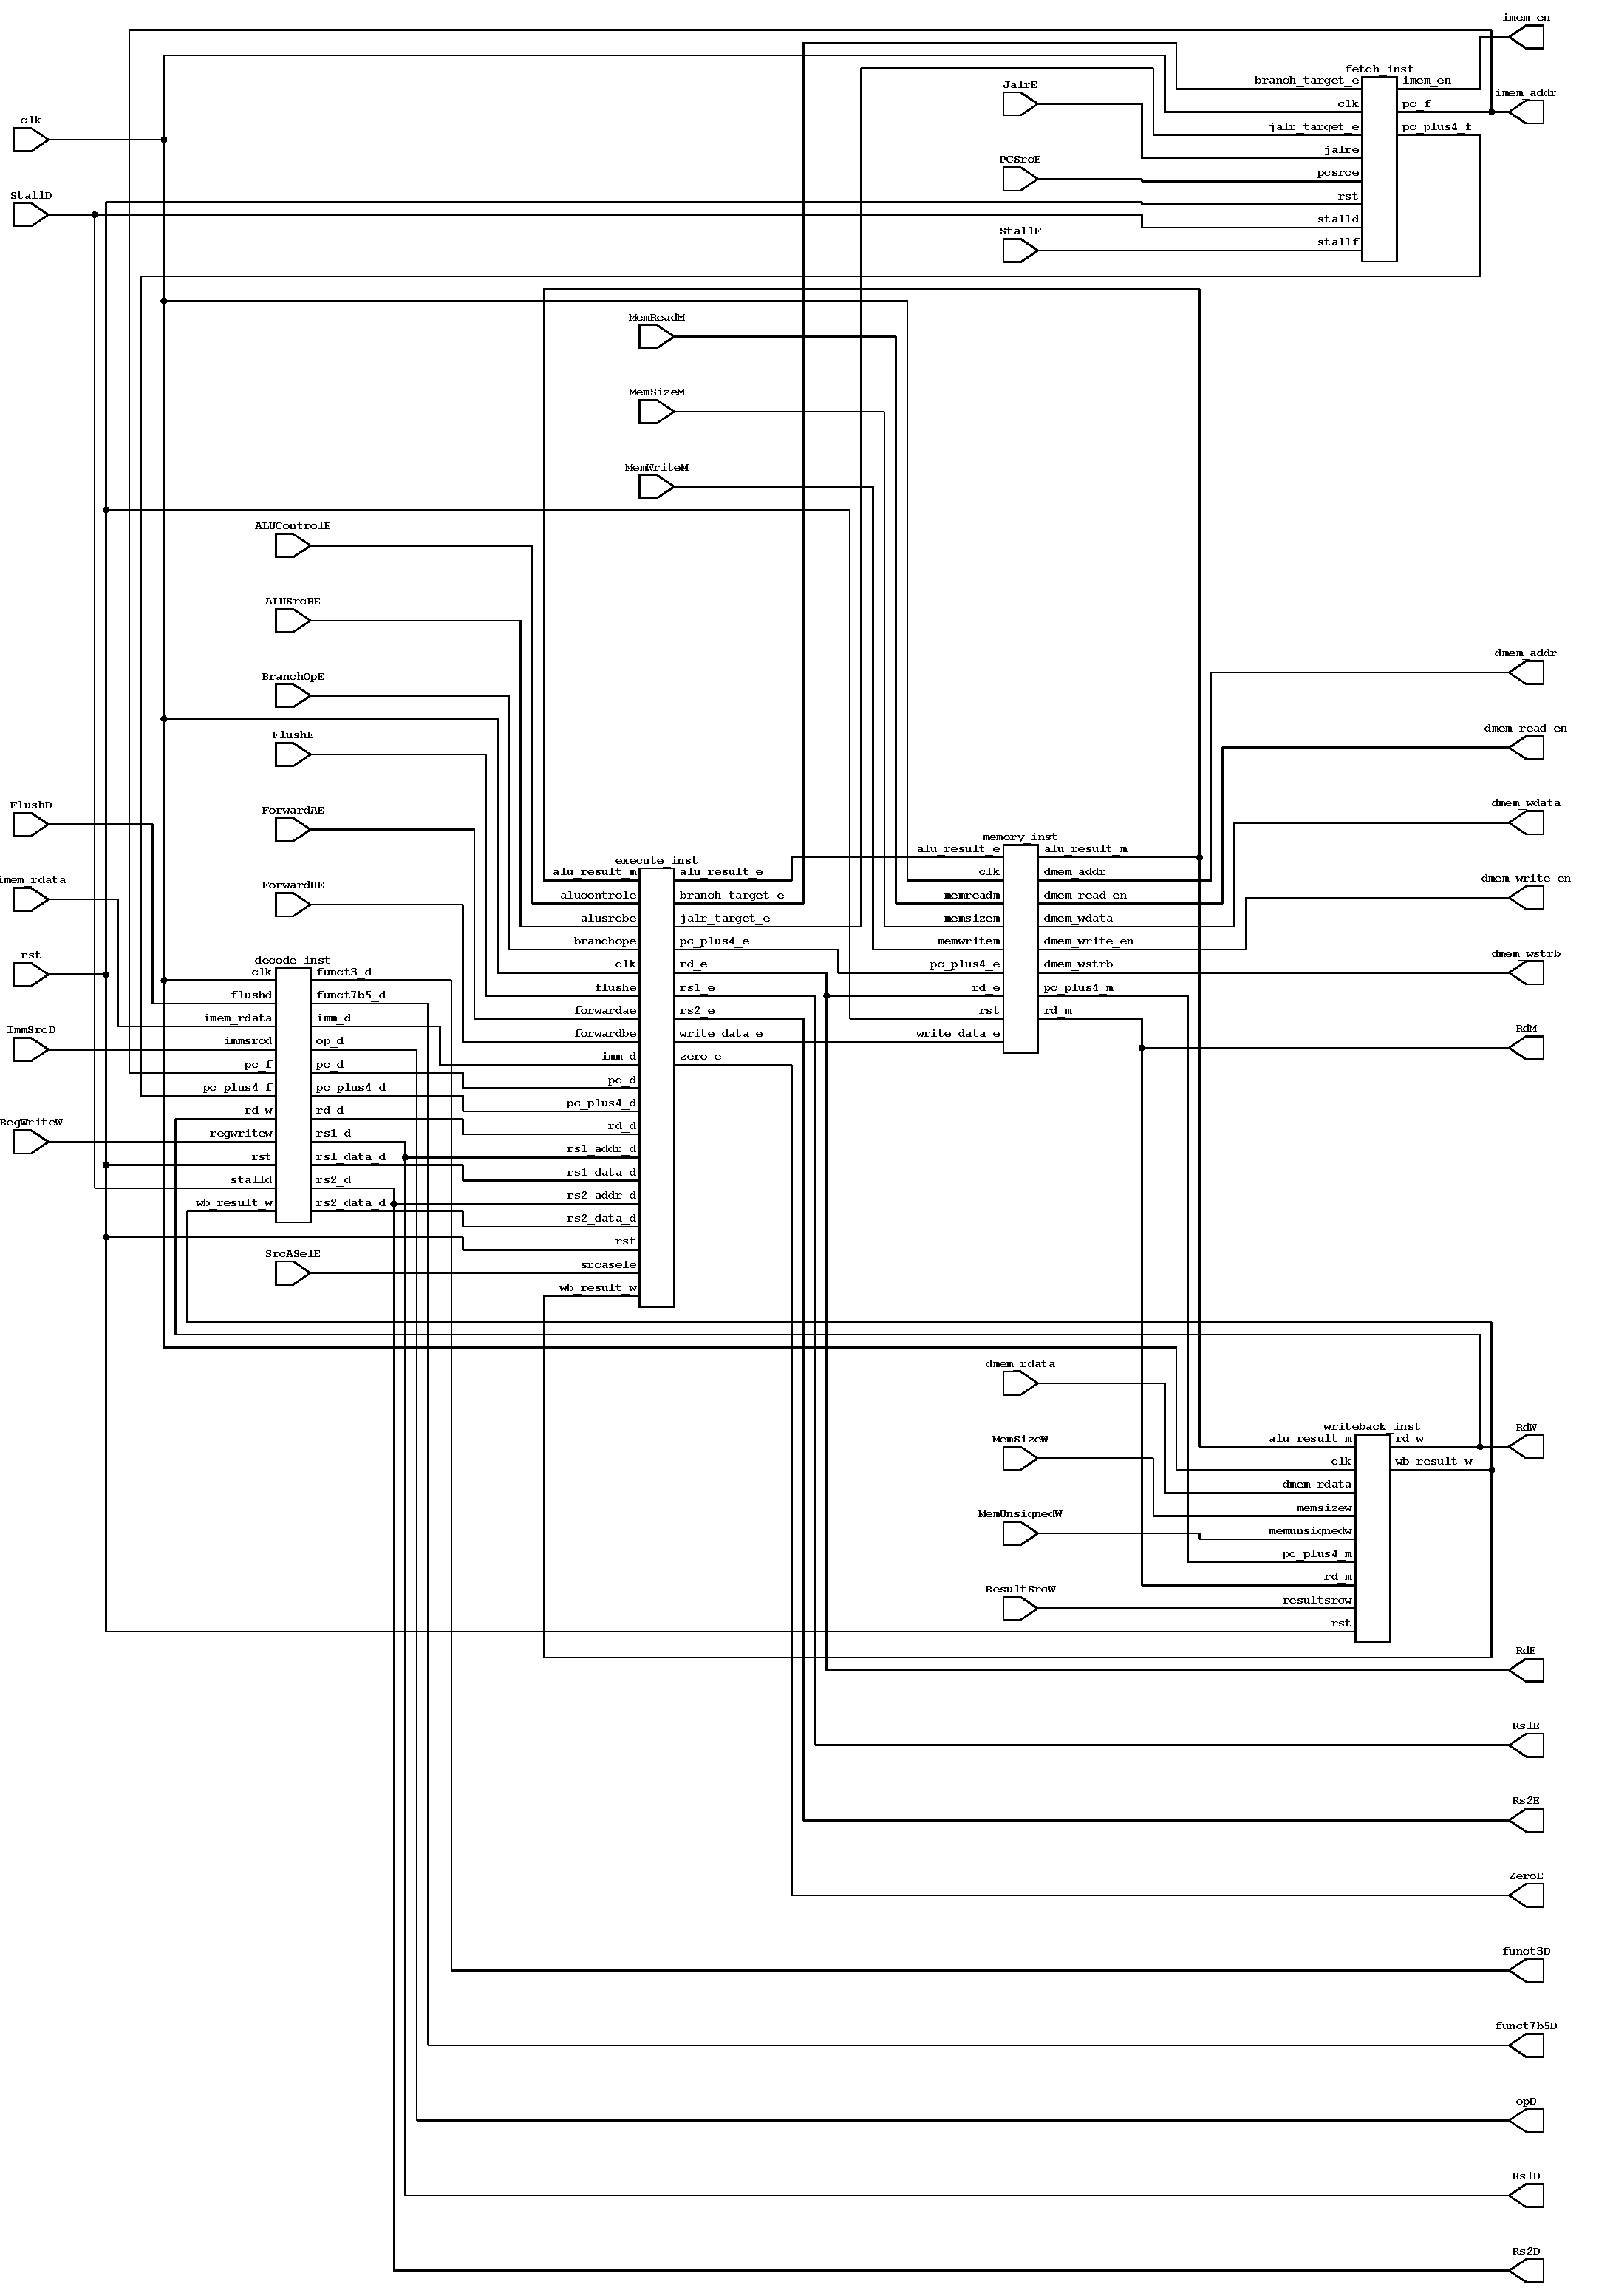
\includegraphics[width=\linewidth,height=0.88\textheight,keepaspectratio]{uarch_stages.pdf}
  \caption{Datapath stages (\texttt{datapath\_pipe}). The purely structural
  datapath instantiates the five per-stage wrappers (\texttt{fetch\_inst},
  \texttt{decode\_inst}, \texttt{execute\_inst}, \texttt{memory\_inst},
  \texttt{writeback\_inst}) and wires the inter-stage signals between them.
  Auto-generated with \texttt{netlistsvg}.}
  \label{fig:uarch-stages}
\end{figure}

\begin{figure}[p]
  \centering
  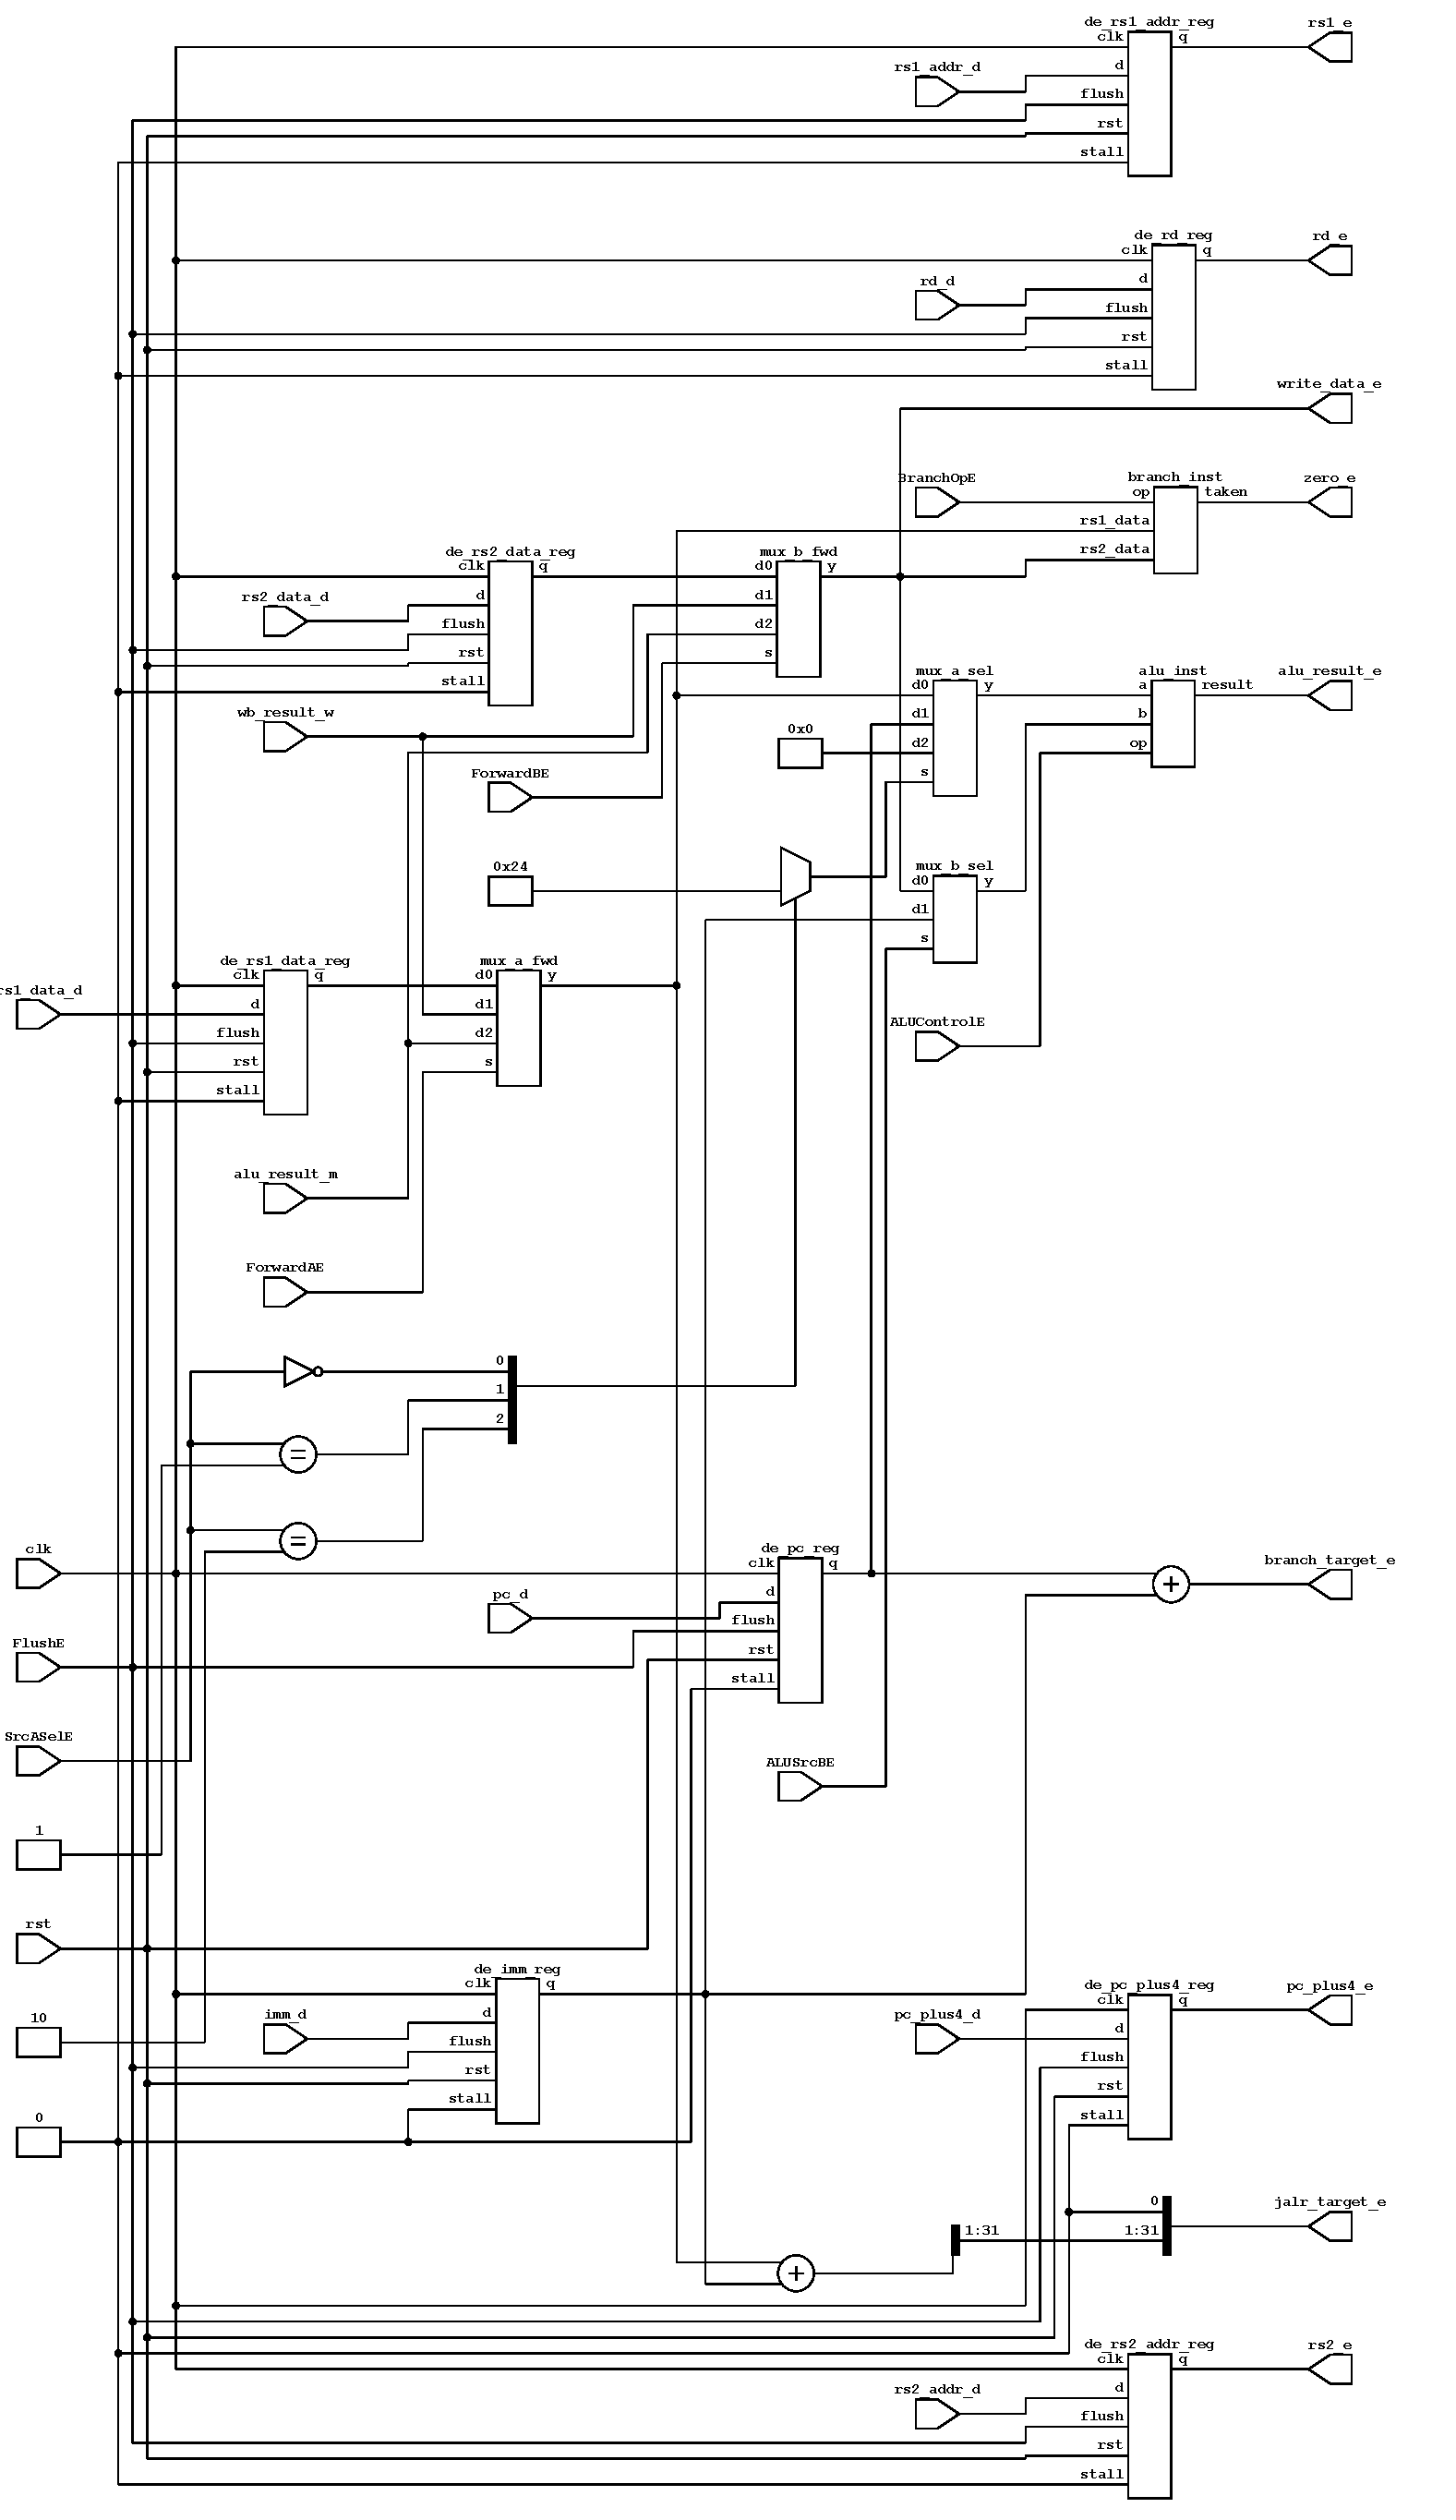
\includegraphics[width=\linewidth,height=0.88\textheight,keepaspectratio]{uarch_execute.pdf}
  \caption{Execute-stage internals (\texttt{execute\_stage}), showing the named
  functional units: the ALU (\texttt{alu\_inst}), the branch unit
  (\texttt{branch\_inst}), the forwarding and operand-select muxes
  (\texttt{mux\_a\_fwd}/\texttt{mux\_b\_fwd}, \texttt{mux\_a\_sel}/\texttt{mux\_b\_sel}),
  the D$\rightarrow$E pipeline registers (\texttt{de\_*\_reg}), and the
  branch-target adder. Auto-generated with \texttt{netlistsvg}.}
  \label{fig:uarch-execute}
\end{figure}

\paragraph{Per-instruction stage walkthrough}
The repository keeps a stage-by-stage walkthrough for each supported RV32I
instruction group in \texttt{docs/instruction\_control.md}. This PDF references
that Markdown source to avoid duplicating the same table-level material in two
places.

\subsection{Major RTL blocks (module map)}
At the core level, \texttt{riscvpipe} binds three blocks
(Figure~\ref{fig:uarch-core}): the controller, the structural datapath, and the
hazard unit.

The design is intentionally modular:
\begin{itemize}[leftmargin=*]
  \item \texttt{riscvpipe.vhd}: binds controller, datapath, and hazard unit into the pipelined core.
  \item \texttt{top.vhd}: wires the core to Harvard IMEM/DMEM models, including \texttt{.rodata} reads via dual-port IMEM. Exposes textbook observation ports (\texttt{DataAdr}, \texttt{WriteData}, \texttt{MemWrite}, \texttt{MemRead}, \texttt{MemWStrb}) so the VHDL testbench can monitor memory traffic directly.
  \item \texttt{fpga\_top.vhd}: thin Vivado synthesis wrapper around \texttt{top}. Exposes \texttt{clk}, \texttt{reset}, and a 1-bit \texttt{led} activity indicator (the MSB of a free-running blink counter XORed with an XOR reduction of every observation signal; the counter makes the LED blink while the clock runs, and the XOR fold prevents Vivado from eliminating the datapath as dead code). It also makes the core clock from the board clock with an MMCM (the FPGA's clock generator block; by default 80\,MHz on Basys3 and ZedBoard). The FPGA pad ring stays at 3 IOs; internal observation nets remain accessible via ILA with \texttt{MARK\_DEBUG}.
  \item \texttt{controller\_pipe.vhd}: decode in D; registers control into E/M/W.
  \item \texttt{datapath\_pipe.vhd}: \textbf{structural} top-level datapath that instantiates five per-stage wrapper entities and wires inter-stage signals (no inline processes or logic).
  \item \texttt{hazard\_unit.vhd}: forwarding, load-use stalls, and control-hazard flush.
  \item \texttt{imem\_dp.vhd}, \texttt{dmem.vhd}: synchronous-read memories coded to infer FPGA BRAM.
  \item \texttt{mem\_access\_unit.vhd}: SB/SH/SW byte strobes + store alignment.
  \item \texttt{load\_extend\_unit.vhd}: combinational load-data sign/zero extension applied in W.
\end{itemize}

\paragraph{Datapath stage hierarchy}
\texttt{datapath\_pipe.vhd} instantiates the following stage wrappers, each
containing named entity instances for pipeline registers (\texttt{pipe\_reg}),
muxes, and functional units.  This produces a navigable per-stage hierarchy in
Vivado's elaborated design view.
\begin{description}[leftmargin=*,labelwidth=3.2cm]
  \item[\texttt{fetch\_stage}] PC register (\texttt{pipe\_reg}), PC+4 adder, next-PC muxes, BRAM read-enable.
  \item[\texttt{decode\_stage}] F$\rightarrow$D pipeline registers, NOP insertion (\texttt{flush\_d\_hold}), \texttt{regfile}, \texttt{extend}.
  \item[\texttt{execute\_stage}] D$\rightarrow$E pipeline registers, forwarding \texttt{mux3} instances, ALU-B \texttt{mux2}, \texttt{alu}, \texttt{branch\_unit}, target computation.
  \item[\texttt{memory\_stage}] E$\rightarrow$M pipeline registers, \texttt{mem\_access\_unit}.
  \item[\texttt{writeback\_stage}] M$\rightarrow$W pipeline registers, \texttt{load\_extend\_unit}, WB result \texttt{mux3}.
\end{description}
A reusable \texttt{pipe\_reg} entity (generic \texttt{WIDTH}, ports for
\texttt{clk/rst/flush/stall/d/q}) implements all explicit pipeline registers.

\subsection{Hazard unit operation}
The hazard unit resolves the three hazard classes of a 5-stage pipeline. A
single elaboration-time generic, \texttt{FORWARDING\_ENABLE}, selects one of
two mutually exclusive bodies through an \texttt{if \ldots generate}. The
stall and flush \emph{outputs} (\texttt{StallF}, \texttt{StallD},
\texttt{FlushD}, \texttt{FlushE}) are produced by shared logic that is
identical in both modes; only the internal stall condition
(\texttt{stallD\_i}) and the forwarding muxes differ between them. The goal of
this subsection is to explain \emph{why each condition is required}, not merely
what it computes.

\subsubsection{Forwarding-enabled mode}
The operand-forwarding muxes choose, for the instruction in Execute, where each
ALU input comes from:

\begin{center}
\begin{tabular}{@{}llp{0.52\textwidth}@{}}
\toprule
Select & Source & Asserted when \\
\midrule
\texttt{"00"} & register file & no hazard, or source is \texttt{x0} (default) \\
\texttt{"10"} & \texttt{ALUResultM} & \texttt{RsxE=RdM} and \texttt{RegWriteM='1'} and \texttt{MemReadM='0'} and \texttt{RsxE/=x0} \\
\texttt{"01"} & \texttt{ResultW}    & \texttt{RsxE=RdW} and \texttt{RegWriteW='1'} and \texttt{RsxE/=x0} \\
\bottomrule
\end{tabular}
\end{center}

\begin{itemize}[leftmargin=*]
  \item \textbf{M before W priority.} When the same register is in flight in
  both M and W, the copy in M is the newer write and must win; the
  \texttt{if/elsif} order encodes this.
  \item \textbf{\texttt{MemReadM='0'} on the M path.} A load in M holds only the
  computed \emph{address} in \texttt{ALUResultM}, not its data; forwarding it
  would corrupt the operand. Loads are instead covered by the load-use stall,
  after which the value forwards safely from W. The W path needs no such guard,
  because W always carries the final committed value.
  \item \textbf{\texttt{RsxE/=x0}.} \texttt{x0} is hardwired to zero and is
  never a real dependency.
\end{itemize}

The remaining data hazard is the \emph{load-use} case: a load in E
(\texttt{ResultSrcEb0='1'}) produces its result only at the end of M, too late
to forward into the dependent instruction already in E. The unit stalls F and D
for one cycle and bubbles E; one cycle later the load is in W and forwards
normally:

\begin{lstlisting}[style=minrv]
stallD_i = ResultSrcEb0='1'
           and ( (Rs1D=RdE and Rs1D/=x0) or (Rs2D=RdE and Rs2D/=x0) )
\end{lstlisting}

\noindent The \texttt{/=x0} guards suppress a false stall when the consumer
reads \texttt{x0}.

\subsubsection{Stall-only mode}
For debugging and for demonstrating why forwarding matters, the unit can be
elaborated with \texttt{FORWARDING\_ENABLE=false}; the test scripts expose this.
The forwarding muxes are tied to \texttt{"00"} (the ALU always reads the
register file), so every RAW dependency must be resolved by stalling until the
producer writes back in W. \texttt{stallD\_i} becomes the OR of the load-use
term above and a generic RAW term:

\begin{lstlisting}[style=minrv]
rawStallD_b = (Rs1D=RdE or Rs2D=RdE) and RegWriteE='1' and RdE/=x0
           or (Rs1D=RdM or Rs2D=RdM) and RegWriteM='1' and RdM/=x0
           or (Rs1D=RdW or Rs2D=RdW) and RegWriteW='1' and RdW/=x0
\end{lstlisting}

\begin{itemize}[leftmargin=*]
  \item \textbf{\texttt{RegWrite*='1'}.} Stores and branches reuse the \texttt{Rd}
  bit-field for immediate bits, so a non-zero \texttt{Rd} does not imply a
  register write. Gating on the real control signal avoids stalling on
  non-existent dependencies.
  \item \textbf{\texttt{Rd*/=x0}.} A write to \texttt{x0} is discarded by the
  ISA, so an instruction whose destination is \texttt{x0} is not a producer.
\end{itemize}

\subsubsection{Shared stall and flush outputs}
\begin{lstlisting}[style=minrv]
StallF = stallD_i and not PCSrcE
StallD = stallD_i and not PCSrcE
FlushD = PCSrcE
FlushE = stallD_i or PCSrcE
\end{lstlisting}

\begin{itemize}[leftmargin=*]
  \item \texttt{StallF}/\texttt{StallD} freeze the PC and the F/D register so the
  dependent instruction stays in D until the hazard clears.
  \item \texttt{FlushD=PCSrcE} kills the speculatively fetched instruction in D
  when a branch or jump resolves taken in E.
  \item \texttt{FlushE} bubbles E for either reason: a data stall has frozen D
  (the instruction in E must not re-execute), or a taken branch must squash its
  wrong-path successor in E.
  \item \textbf{The \texttt{and not PCSrcE} guard.} When a taken branch coincides
  with a data stall the PC must still redirect. \texttt{StallF} is the only gate
  on the PC update -- there is no flush on the PC -- so the guard is
  \emph{required} on \texttt{StallF}; without it the PC freezes and the core
  re-fetches the wrong-path instruction indefinitely. On \texttt{StallD} the
  guard is \emph{redundant}: \texttt{FlushD=PCSrcE} already clears the F/D
  register, and \texttt{pipe\_reg} prioritises flush over stall
  (\texttt{rst/flush > stall > load}), so the register bubbles regardless of
  \texttt{StallD}; it is kept only for symmetry. In forwarding mode
  \texttt{stallD\_i} (a load in E) and \texttt{PCSrcE} (a taken branch/jump in E)
  are mutually exclusive, so the guard only ever fires in stall-only mode, where
  a \texttt{JAL}/\texttt{JALR} both writes \texttt{rd} and sets \texttt{PCSrcE}.
\end{itemize}

\clearpage
\section{ISA coverage and control signals}

\subsection{Instruction groups}
The core targets a practical RV32I subset intended to be ``GCC-friendly'' for
freestanding bare-metal programs:
\begin{itemize}[leftmargin=*]
  \item Control flow: JAL, JALR, and all RV32I branches (BEQ/BNE/BLT/BGE/BLTU/BGEU).
  \item Address materialization: LUI, AUIPC.
  \item Loads: LB/LBU, LH/LHU, LW (with sign/zero extension).
  \item Stores: SB/SH/SW (with correct byte-lane strobes and alignment).
  \item Integer ALU: OP-IMM and OP arithmetic/logical instructions (ADD/SUB/AND/OR/XOR/SLT/SLTU/SLL/SRL/SRA and immediate forms).
\end{itemize}

\subsection{Control signal glossary (selected)}
The controller emits decode-stage signals that are registered into E/M/W.
Common signals you will see in waveforms and RTL include:
\begin{itemize}[leftmargin=*]
  \item \texttt{ResultSrcW}: writeback mux select (ALU vs MEM vs PC+4).
  \item \texttt{MemWriteM} / \texttt{MemReadM}: DMEM write/read enables.
  \item \texttt{ImmSrcD}: immediate format (I/S/B/U/J).
  \item \texttt{ALUControlE}, \texttt{SrcASelE}, \texttt{ALUSrcBE}: ALU operation and operand selection.
  \item \texttt{BranchOpE}: branch comparator mode (eq/lt/ltu/etc.).
  \item \texttt{JumpE} / \texttt{JalrE}: unconditional control-flow redirect (JAL/JALR).
  \item \texttt{PCSrcE}: redirect decision (taken branch/jump) that selects the next PC.
\end{itemize}

\subsection{Control naming and stage suffixes}
Control is generated in Decode and registered through E/M/W (for example
\texttt{ImmSrcD}, \texttt{ALUControlE}, \texttt{MemWriteM}, \texttt{ResultSrcW}).
This mirrors the textbook convention while making timing explicit in the RTL.

\subsection{Compact control matrix (from \texttt{docs/instruction\_control.md})}

\paragraph{Execute + writeback}
\begin{center}
\small
\begin{tabular}{@{}l l l l l l l@{}}
\toprule
Group & ImmSrcD & SrcASelE & ALUSrcBE & ALUControlE & RegWriteW & ResultSrcW \\
\midrule
LUI    & IMM\_U & OPA\_ZERO & imm & ALU\_ADD & yes & WB\_ALU \\
AUIPC  & IMM\_U & OPA\_PC   & imm & ALU\_ADD & yes & WB\_ALU \\
JAL    & IMM\_J & OPA\_PC   & imm & ALU\_ADD & yes & WB\_PC4 \\
JALR   & IMM\_I & OPA\_RS1  & imm & ALU\_ADD & yes & WB\_PC4 \\
Branch & IMM\_B & OPA\_RS1  & rs2 & ALU\_SUB & no  & WB\_ALU \\
Load   & IMM\_I & OPA\_RS1  & imm & ALU\_ADD & yes & WB\_MEM \\
Store  & IMM\_S & OPA\_RS1  & imm & ALU\_ADD & no  & WB\_ALU \\
OP-IMM & IMM\_I & OPA\_RS1  & imm & funct   & yes & WB\_ALU \\
OP     & IMM\_I & OPA\_RS1  & rs2 & funct   & yes & WB\_ALU \\
\bottomrule
\end{tabular}
\end{center}
\normalsize

\paragraph{Memory + PC control}
\begin{center}
\small
\begin{tabular}{@{}l c c l l l c c@{}}
\toprule
Group & MemReadM & MemWriteM & MemSizeM & MemUnsignedM & BranchOpE & JumpE & JalrE \\
\midrule
LUI    & 0 & 0 & --   & --    & BR\_NONE & 0 & 0 \\
AUIPC  & 0 & 0 & --   & --    & BR\_NONE & 0 & 0 \\
JAL    & 0 & 0 & --   & --    & BR\_NONE & 1 & 0 \\
JALR   & 0 & 0 & --   & --    & BR\_NONE & 1 & 1 \\
Branch & 0 & 0 & --   & --    & funct    & 0 & 0 \\
Load   & 1 & 0 & size & funct & BR\_NONE & 0 & 0 \\
Store  & 0 & 1 & size & 0     & BR\_NONE & 0 & 0 \\
OP-IMM & 0 & 0 & --   & --    & BR\_NONE & 0 & 0 \\
OP     & 0 & 0 & --   & --    & BR\_NONE & 0 & 0 \\
\bottomrule
\end{tabular}
\end{center}
\normalsize

\clearpage
\section{Memory map, linker script, and GCC-to-hex flow}

\subsection{Harvard memory map}
The RTL models separate instruction and data memories. Software is linked to
match the address split so code and writable data never overlap.

\begin{center}
\begin{tabularx}{\linewidth}{@{}l l l l X@{}}
\toprule
Region & Base address & Size & Access & Purpose \\
\midrule
IMEM & \texttt{0x0000\_0000} & 8 KiB & read/execute & \texttt{.text}, \texttt{.init}, \texttt{.rodata} \\
DMEM & \texttt{0x2000\_0000} & 8 KiB & read/write & \texttt{.data}, \texttt{.sdata}, \texttt{.bss}, stack, signature window \\
\bottomrule
\end{tabularx}
\end{center}

Tests use a fixed signature scratch region at \texttt{0x2000\_0100}: programs
write deterministic 32-bit words there, and the testbench compares them against
golden \texttt{.sig} files.

\subsection{Why these addresses?}
The documentation emphasizes a few motivations:
\begin{itemize}[leftmargin=*]
  \item The PC resets to zero, so placing IMEM at \texttt{0x0000\_0000} makes reset-to-first-instruction trivial.
  \item The DMEM base at \texttt{0x2000\_0000} makes the Harvard split obvious from the address, and leaves room to grow toward a small SoC/MMIO map.
  \item The linker fixes a deterministic stack top and a deterministic signature window for self-checking tests.
\end{itemize}

\subsection{A note on address decoding in the simple memories}
The VHDL \texttt{imem\_dp} and \texttt{dmem} models intentionally do not
implement full high-bit address decode; they mask down to the configured depth
when indexing their arrays. The
software \emph{still} uses full logical addresses (IMEM at \texttt{0x0000\_xxxx},
DMEM at \texttt{0x2000\_xxxx}) so that the linker keeps sections separated.
When integrating into a larger system, you can wrap proper decode logic around
the memories without changing the compiler/linker view.

\subsection{Data-side reads from the text region (\texttt{.rodata})}
Because \texttt{.rodata} constants are placed in IMEM alongside \texttt{.text},
loads that target addresses below \texttt{DMEM\_BASE\_ADDR}
(\texttt{0x2000\_0000}) must read from IMEM, not DMEM. The top-level wrapper
\texttt{top.vhd} instantiates a true dual-port instruction memory
(\texttt{imem\_dp}): port A serves instruction fetch and port B serves data-side
reads. A registered mux-select (\texttt{use\_imem\_w}) aligns the IMEM/DMEM
read-data mux with the synchronous BRAM output timing.

\subsection{Linker script (\texttt{link.ld})}
The provided linker script enforces the memory map:
\begin{itemize}[leftmargin=*]
  \item \texttt{.text} and \texttt{.rodata} go to IMEM at \texttt{0x0000\_0000} (the PC resets to zero).
  \item \texttt{.data} (and small-data \texttt{.sdata}) live in DMEM at runtime but are placed \emph{in the ELF load image} so the build can initialize DMEM before releasing reset.
  \item \texttt{.bss} (and \texttt{.sbss}) are zero-initialized at runtime and do not need hex initialization data.
  \item \texttt{\_\_stack\_top} is set to the top of DMEM so freestanding startup code can initialize \texttt{sp}.
  \item \texttt{.note} sections are discarded, and the link stops with an error if \texttt{.text} does not start at \texttt{0x0000\_0000}. Some toolchains, for example the RISC-V GCC that comes with AMD Vitis, add a build-ID note section by default; placed in front of \texttt{.text}, it would move the code away from the address where the IMEM image starts.
\end{itemize}

\paragraph{Key snippet}
\begin{lstlisting}[style=minrv]
MEMORY {
  IMEM (rx) : ORIGIN = 0x00000000, LENGTH = 8K
  DMEM (rw) : ORIGIN = 0x20000000, LENGTH = 8K
}
\end{lstlisting}

\paragraph{Spike variant (\texttt{link\_spike.ld})}
The golden signatures are generated on the Spike ISA simulator
(Section~\ref{sec:spike-golden}). Spike reserves the low addresses for its debug
module and boot ROM, so \texttt{link\_spike.ld} places the code at
\texttt{0x8000\_0000} and keeps DMEM, the stack, and the signature window at
their MinRV32 addresses. \texttt{.data} is placed at its run address, so Spike's
ELF loader preloads DMEM as \texttt{<name>.data.hex} does on the core.
\texttt{build\_prog.sh} selects it through the \texttt{LINKER\_SCRIPT}
environment variable. Section~\ref{sec:spike-addr} explains which signature
values this affects.

\subsection{GCC $\rightarrow$ ELF $\rightarrow$ hex images}
The project's workflow emphasizes real software running on the RTL:
\begin{enumerate}[leftmargin=*]
  \item Compile/link a freestanding RV32I program with a bare-metal RISC-V GCC toolchain.
  \item Extract \texttt{.text/.rodata} and \texttt{.data/.sdata} into raw binaries via \texttt{objcopy}.
  \item Convert those binaries into newline-delimited 32-bit hex words (\texttt{XXXXXXXX} per line) for IMEM/DMEM initialization.
\end{enumerate}

The helper script \texttt{scripts/build\_prog.sh} automates this and produces:
\texttt{<base>.elf}, \texttt{<base>.text.hex}, \texttt{<base>.data.hex} (and, for
C sources, a compiler-generated assembly listing \texttt{<base>.S}).

\paragraph{Practical guard: do the images fit?}
The educational memories are small (default 8\,KiB IMEM and 8\,KiB DMEM). The build script
prints a size summary for the generated \texttt{.text} and \texttt{.data} images
and emits warnings if either exceeds the configured IMEM/DMEM capacity. If you
change the VHDL memory sizes, set \texttt{IMEM\_BYTES} and \texttt{DMEM\_BYTES}
in the environment so the warnings match your configuration.

\subsection{Future work: one memory map for the core and Spike}
\label{sec:future-memmap}
The two linker scripts exist only because the core's IMEM sits at
\texttt{0x0}, where Spike has its debug module. Spike does not accept memory
there. Its other devices (boot ROM at \texttt{0x1000}, CLINT at
\texttt{0x0200\_0000}, PLIC at \texttt{0x0C00\_0000}, UART at
\texttt{0x1000\_0000}) do not overlap DMEM at \texttt{0x2000\_0000}. If IMEM
and the reset PC move to \texttt{0x8000\_0000} (the RAM base also used by
riscv-tests, riscv-arch-test, QEMU \texttt{virt}, and Sail), one linker script
serves both. DMEM, the stack, and the signature window do not change. The
current layout does not affect the golden signatures as long as tests follow
the code-address rule (Section~\ref{sec:spike-addr}), so this change is not
needed now. Required changes:
\begin{enumerate}[leftmargin=*]
  \item \textbf{Reset PC.} Add a reset-value generic to \texttt{pipe\_reg}
  (default zero) and a \texttt{RESET\_PC} generic (default
  \texttt{x"80000000"}) passed down to \texttt{pc\_reg} in
  \texttt{fetch\_stage}.
  \item \textbf{Load-path decode.} \texttt{top.vhd} and
  \texttt{sim/top\_trace.vhd} send a load to IMEM port~B when
  \texttt{addr < DMEM\_BASE\_ADDR}; test address bit~31 instead (set for
  IMEM, clear for DMEM), which also needs less logic.
  \item \textbf{Memories.} No change: \texttt{imem\_dp} and \texttt{dmem} index
  only the low address bits.
  \item \textbf{Linker script.} Set \texttt{IMEM ORIGIN = 0x80000000} in
  \texttt{link.ld} and remove \texttt{AT>IMEM} (nothing copies \texttt{.data}
  from its load address). Delete \texttt{link\_spike.ld} and the
  \texttt{LINKER\_SCRIPT} override in \texttt{gen\_golden.sh}.
  \item \textbf{Documentation.} Update the address tables, remove the
  code-address rule, and update examples that show PC values.
\end{enumerate}
Raw code addresses would then give the same signature on both, and the existing
\texttt{.sig} files stay valid. The PC would no longer reset to zero. The
differences in Section~\ref{sec:spike-other} remain.

\clearpage
\section{Directed instruction tests and helper scripts}

\subsection{ISA tests}
Directed tests under \texttt{tests/isa/} exercise every supported instruction
group. Each test writes a deterministic signature to \texttt{0x2000\_0100} and
ships with a golden \texttt{.sig} file. The golden words are generated with the
Spike RISC-V ISA simulator (Section~\ref{sec:spike-golden}).

\subsection{Prerequisites}
The documented workflow assumes:
\begin{itemize}[leftmargin=*]
  \item A bare-metal RISC-V GCC toolchain (e.g. \texttt{riscv64-unknown-elf-gcc} and \texttt{objcopy}).
  \item Python 3 (used for binary-to-hex conversion).
  \item GHDL with VHDL-2008 support (for simulation).
\end{itemize}

On Ubuntu, the documentation suggests installing the basics via APT:
\begin{lstlisting}[style=minrv]
sudo apt update
sudo apt install gcc-riscv64-unknown-elf binutils-riscv64-unknown-elf \
  ghdl python3 python3-pip make
\end{lstlisting}

\paragraph{Optional: Spike (golden signatures)}
\texttt{gen\_golden.sh} and \texttt{check\_goldens.sh} need the Spike ISA
simulator. Spike is not packaged for Ubuntu, so it is built from source:
\begin{lstlisting}[style=minrv]
sudo apt install -y build-essential git device-tree-compiler \
  libboost-regex-dev libboost-system-dev
git clone https://github.com/riscv-software-src/riscv-isa-sim.git
cd riscv-isa-sim && mkdir build && cd build
../configure --prefix=/opt/riscv   # or --prefix=$HOME/.local (no sudo)
make -j"$(nproc)" && sudo make install
export PATH=/opt/riscv/bin:$PATH
spike --help | grep debug-cmd      # check
\end{lstlisting}
Spike is needed only to create or re-check \texttt{.sig} files, not to run the
existing tests.

\paragraph{Optional: schematic generation and DigitalJS interactive simulation}
To generate SVG schematics of RTL entities and to export DigitalJS JSON for
interactive browser-based simulation (see \texttt{scripts/gen\_schematic.sh}):
\begin{lstlisting}[style=minrv]
sudo apt install -y yosys ghdl yosys-plugin-ghdl graphviz
sudo apt install -y nodejs npm
sudo npm install -g netlistsvg
sudo npm install -g yosys2digitaljs
\end{lstlisting}

\subsection{One-test and batch workflows}
The repository provides scripts that build programs (using GCC) and run the
self-checking testbench (GHDL):

\begin{lstlisting}[style=minrv]
./scripts/run_test.sh full_core
./scripts/run_test.sh --trace full_core
./scripts/run_test.sh --fst full_core
./scripts/run_tests.sh
./scripts/run_tests.sh --trace
\end{lstlisting}

Useful environment overrides include \texttt{MAX\_CYCLES} (for longer programs),
\texttt{FORWARDING\_ENABLE=false} (stall-only hazards), and tool-path variables
such as \texttt{RISCV\_GCC} and \texttt{RISCV\_OBJCOPY}. For simulation, the
scripts also honor \texttt{GHDL} and \texttt{GHDL\_STD} and provide a
\texttt{--verbose}/\texttt{VERBOSE=1} mode to echo the underlying GHDL commands.
To keep the repository root clean (and to avoid collisions when running multiple
tests in parallel), the scripts isolate GHDL work libraries and elaboration
executables under \texttt{build/ghdl/} by default (override with
\texttt{GHDL\_WORKDIR}).

\subsection{Waveform dumps (GTKWave)}
For waveform-first debugging, the scripts can dump waveforms directly from GHDL:
\begin{itemize}[leftmargin=*]
  \item \texttt{--fst}: fast, compact waveform format (recommended).
  \item \texttt{--vcd}: widely supported text waveform.
  \item \texttt{--wave}: GHDL's \texttt{.ghw} format.
\end{itemize}

\begin{lstlisting}[style=minrv]
./scripts/run_test.sh --fst addi_only
./scripts/view_wave.sh build/waves/addi_only.fst
\end{lstlisting}

\subsection{Unit-level testbenches}
For component bring-up without building a program image, run unit testbenches:
\begin{lstlisting}[style=minrv]
./scripts/run_unit_tb.sh regfile
./scripts/run_unit_tb.sh --fst alu
\end{lstlisting}

\subsection{DigitalJS interactive simulation}
\label{sec:digitaljs}
\texttt{gen\_schematic.sh --digitaljs} exports a DigitalJS-compatible JSON that you
can upload to \url{https://digitaljs.tilk.eu/}.  DigitalJS is both a schematic
viewer \emph{and} an interactive simulator: you drive inputs by clicking and watch
values propagate through the gates.  It acts as a visual complement to GTKWave
(for leaf modules) and to the GHDL full-core tests (for the whole pipeline).  It
is not a replacement for the signature-checked \texttt{run\_test.sh} /
\texttt{run\_tests.sh} flows -- those remain the authoritative pass/fail.

\paragraph{Automatic clock and reset ergonomics}
The \texttt{--digitaljs} post-processor calls \texttt{yosys2digitaljs}'s
\texttt{io\_ui()} helper, which remaps raw port devices into simulator-UI
widgets so the exported circuit is immediately runnable without manual clock
toggling: a 1-bit \texttt{Input} named \texttt{clk} becomes a
self-ticking \texttt{Clock} device, any other 1-bit \texttt{Input} (e.g.
\texttt{reset}) becomes a one-click \texttt{Button}, multi-bit \texttt{Input}s
become \texttt{NumEntry} typeable fields, and outputs become \texttt{Lamp} /
\texttt{NumDisplay}.  Upload, press the simulator's run button (auto-pressed by default when loading the .json file), and click
\texttt{reset} once and then click again to create a reset pulse -- the clock runs on its own.

\paragraph{Simple modules (leaf entities)}
Export a single entity and open it in DigitalJS:
\begin{lstlisting}[style=minrv]
./scripts/gen_schematic.sh --digitaljs alu
./scripts/gen_schematic.sh --digitaljs regfile
./scripts/gen_schematic.sh --digitaljs extend
\end{lstlisting}
Upload \texttt{build/schematics/<entity>.digitaljs.json} and toggle inputs.

\paragraph{Full pipeline with real firmware (\texttt{--mem-init})}
Yosys synthesis excludes the \texttt{synthesis translate\_off} guards in
\texttt{mem\_init\_pkg.vhd}, so every memory cell in the exported netlist has
an all-zero initial state.  The \texttt{--mem-init} flag patches the
\texttt{\$mem}/\texttt{\$mem\_v2} INIT parameter with the real hex images
before \texttt{yosys2digitaljs} converts the netlist, giving the DigitalJS
interactive simulation a faithful firmware image:
\begin{lstlisting}[style=minrv]
./scripts/build_prog.sh tests/isa/full_core.c full_core
./scripts/gen_schematic.sh --digitaljs \
    --mem-init imem_dp=build/full_core.text.hex \
    --mem-init dmem=build/full_core.data.hex \
    top
\end{lstlisting}
Upload the resulting \texttt{build/schematics/top.digitaljs.json} to
\url{https://digitaljs.tilk.eu/} to step through the pipeline with the program
already loaded in memory (Figure~\ref{fig:digitaljs-top}).  The
\texttt{--mem-init} injection only works on the
hierarchical (default) netlist where \texttt{imem\_dp} and \texttt{dmem} are
distinct modules; under \texttt{--flat} the modules merge into the top level
and the injection becomes a no-op (a warning is printed).

\begin{figure}[ht]
  \centering
  \fbox{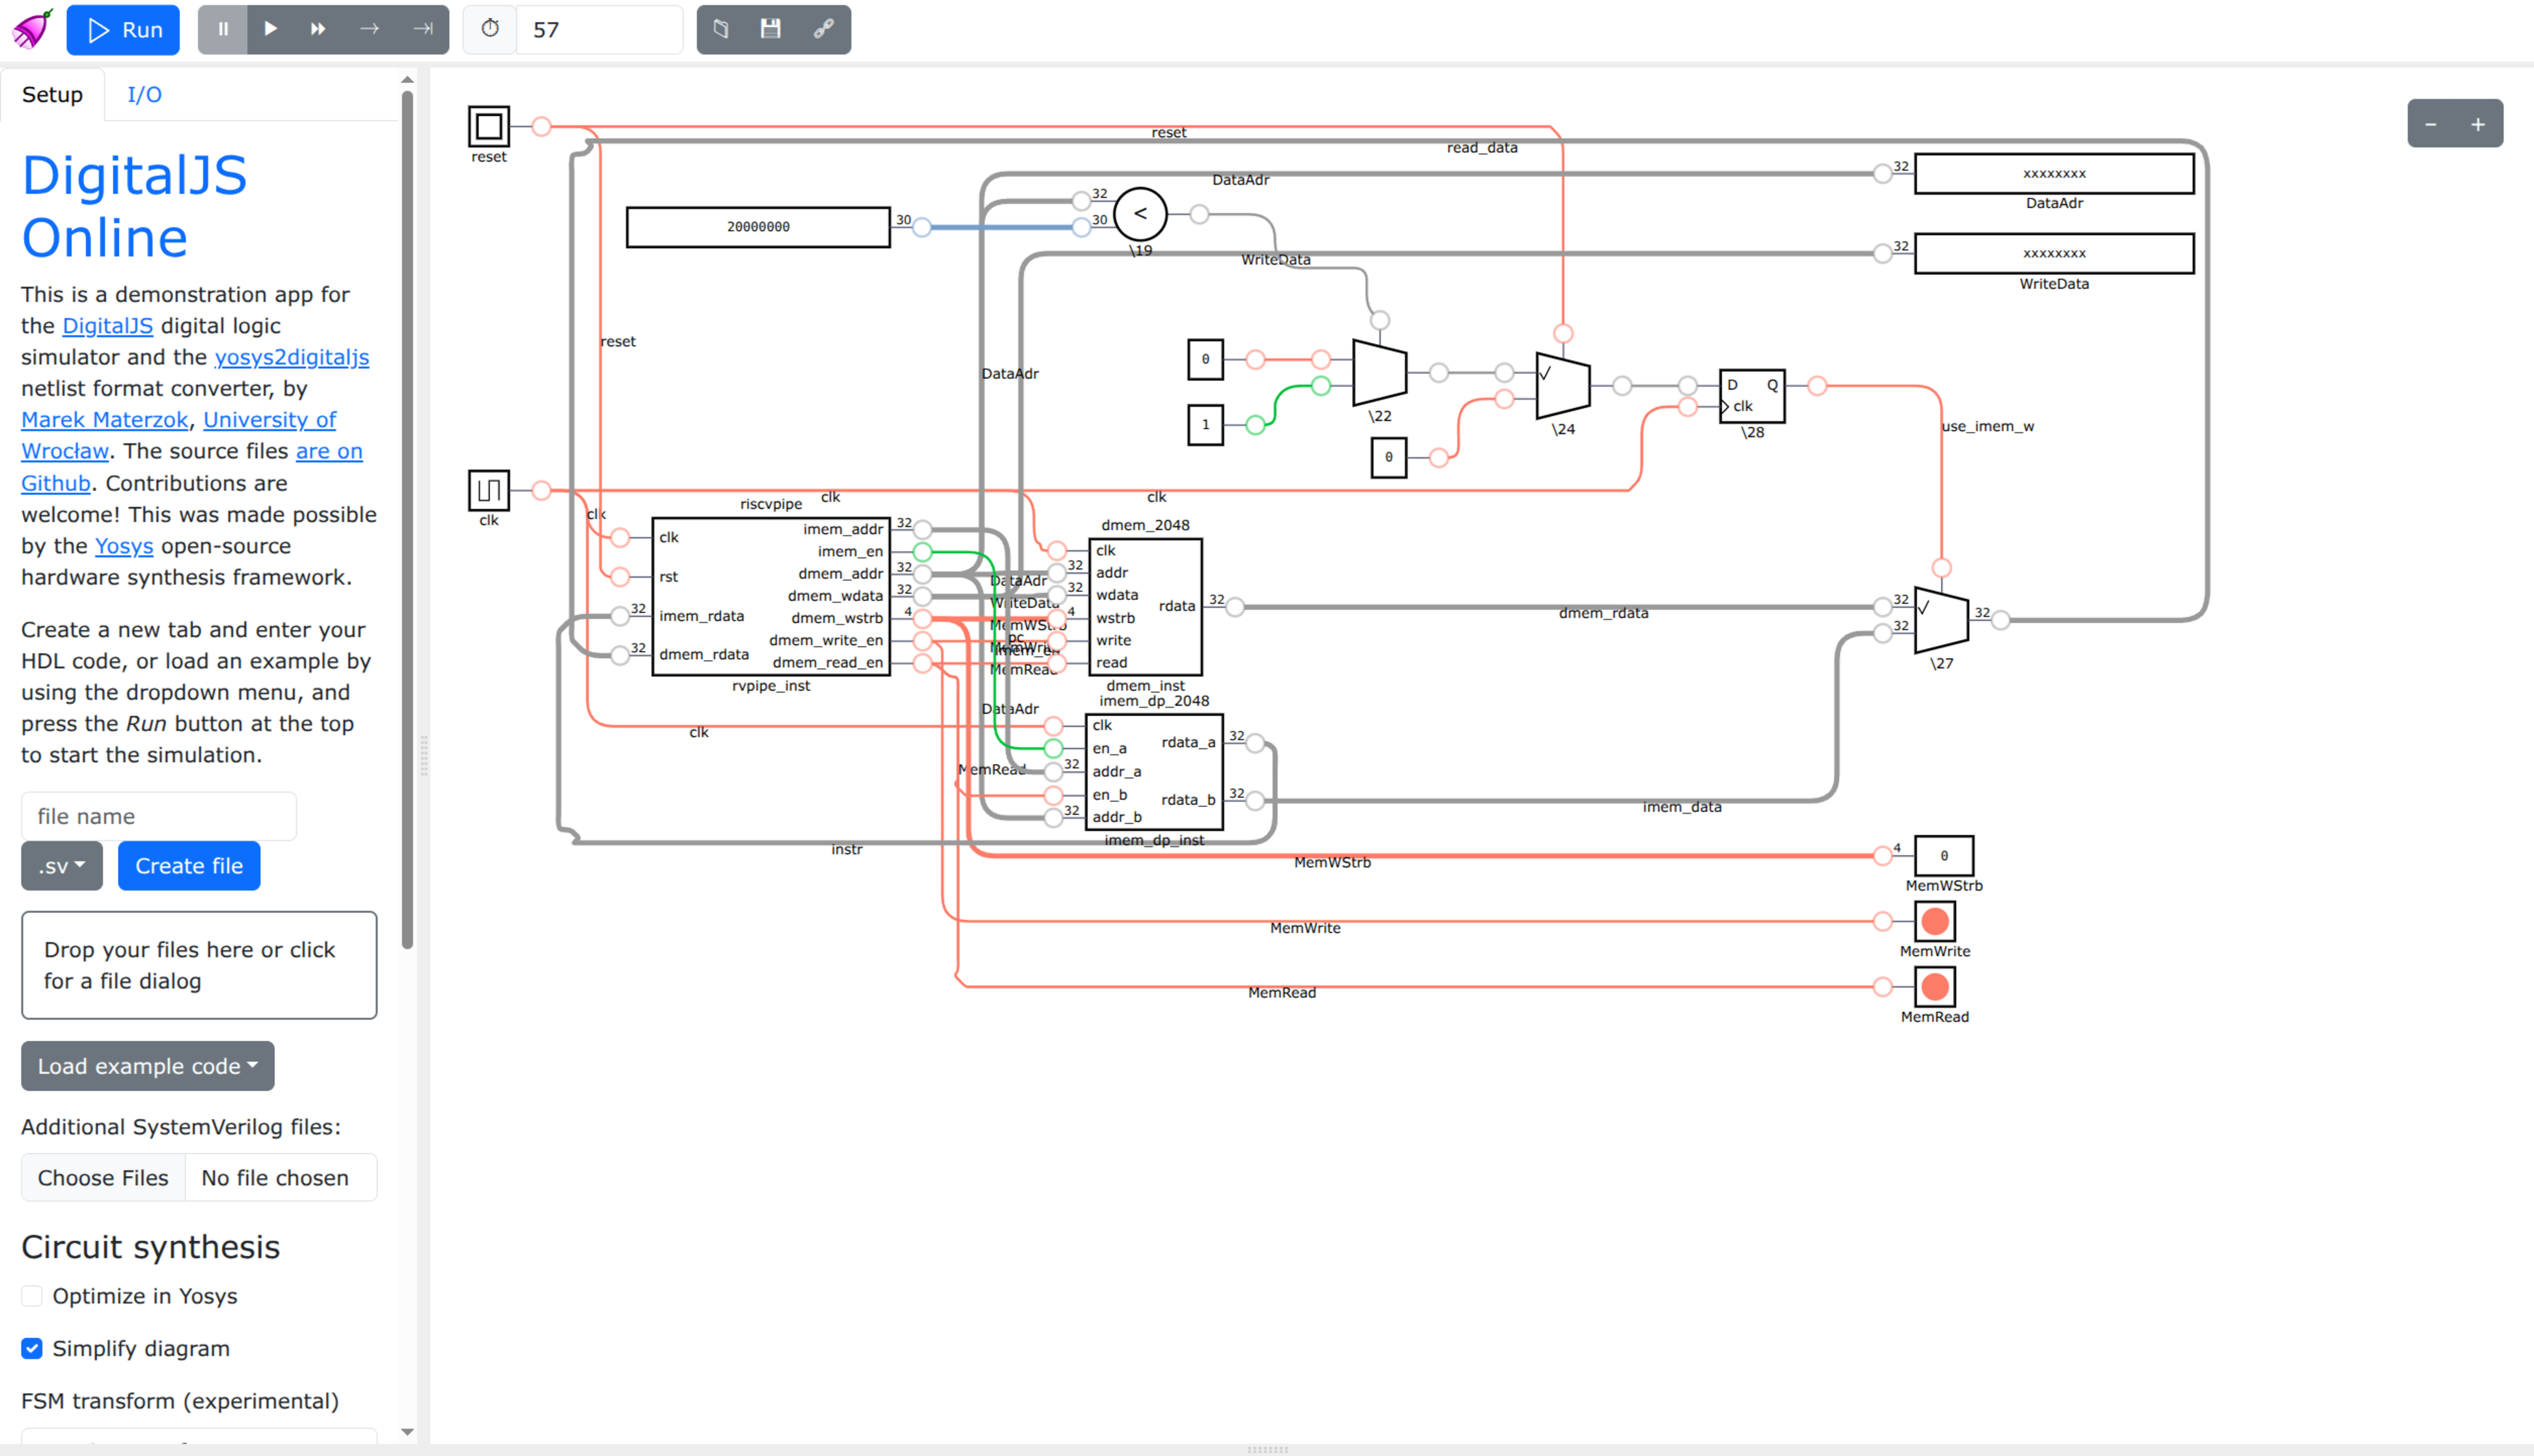
\includegraphics[scale=0.18]{digitaljs-top.pdf}}
  \caption{DigitalJS simulation of the full\_core.c program running on MinRV32.}
  \label{fig:digitaljs-top}
\end{figure}

\subsection{Trace output (optional)}
Both the GHDL-driven scripts and the Vivado documentation describe an optional
per-instruction trace that prints decoded assembly and key control selections
grouped by stage. This is designed as a teaching aid: it links what the program
is doing (assembly) to what the controller and hazard logic are doing (mux and
enable choices).

When the hazard unit takes action (stall/flush/forward), the trace prints an
additional \texttt{HAZARD:} line showing stall/flush decisions plus the
forwarding-source selects for the E-stage operands:
\begin{lstlisting}[style=minrv]
HAZARD: StallF=stall StallD=stall FlushD=keep FlushE=flush FwdA=rf FwdB=rf
\end{lstlisting}
\noindent
\texttt{FwdA/FwdB} select \texttt{rf} (regfile), \texttt{M} (Memory stage), or
\texttt{W} (Writeback stage). The hazard line is only printed when something is
asserted or forwarded.

\subsection{Authoring new tests}
New tests can be written as assembly (\texttt{.S}) or freestanding C
(\texttt{.c}) under \texttt{tests/isa/}. The expected flow is:
\begin{enumerate}[leftmargin=*]
  \item Write a deterministic workload using only the supported instruction subset.
  \item Write final observation words into the signature buffer at \texttt{0x2000\_0100}.
  \item Generate the golden signature with Spike:
  \texttt{./scripts/gen\_golden.sh --words N --write <name>} runs the same
  program on the Spike reference model, reads \texttt{N} words from the signature
  window at \texttt{0x2000\_0100}, and writes \texttt{tests/isa/<name>.sig}
  (Section~\ref{sec:spike-golden}). Do not store raw code or \texttt{.rodata}
  addresses in the signature (Section~\ref{sec:spike-addr}). (Compiling the C for
  the host x86 architecture is \emph{not} a reliable oracle, since 32-bit
  overflow and shift semantics may differ from RV32I.)
  \item Re-run via \texttt{scripts/run\_test.sh <name>} for regression.
\end{enumerate}

\subsection{Golden signatures with Spike}
\label{sec:spike-golden}
The expected \texttt{.sig} words come from Spike, the RISC-V reference ISA
simulator. Spike does not depend on the RTL, so it is an independent oracle for
the design under test.
\begin{lstlisting}[style=minrv]
./scripts/gen_golden.sh factorial                 # print, save build/golden/factorial.sig
./scripts/gen_golden.sh --check factorial         # compare with tests/isa/factorial.sig
./scripts/gen_golden.sh --words 4 --write my_test # create tests/isa/my_test.sig
./scripts/check_goldens.sh                        # check every tests/isa/*.sig
\end{lstlisting}
\texttt{gen\_golden.sh} builds the test with \texttt{build\_prog.sh} (same
compiler flags as the core) and the linker script \texttt{link\_spike.ld}. It
runs the ELF on Spike in debug mode for \texttt{SPIKE\_MAX\_INSNS} instructions
(default 1\,000\,000) and checks that the PC is parked in the final self-loop.
It then reads the signature window and writes \texttt{build/golden/<name>.sig},
one lowercase hex word per line. The word count is \texttt{--words N} or the
line count of the existing \texttt{.sig} file. \texttt{--write} copies the result
to \texttt{tests/isa/<name>.sig}, and \texttt{--check} compares it with that
file. \texttt{check\_goldens.sh} runs \texttt{--check} for every test. The
environment variables \texttt{SPIKE}, \texttt{SPIKE\_ISA} (default
\texttt{rv32i}), and \texttt{SPIKE\_MAX\_INSNS} select the binary, the ISA
string, and the instruction budget.

\paragraph{Spike vs MinRV32 code addresses}
\label{sec:spike-addr}
Spike reserves the low address space for its debug module
(\texttt{0x0000\_0000}--\texttt{0x0000\_0FFF}) and boot ROM (from
\texttt{0x1000}), so instruction memory cannot sit at \texttt{0x0} as it does on
MinRV32. \texttt{link\_spike.ld} moves the code to \texttt{0x8000\_0000};
data memory does not move.

\begin{center}
\begin{tabularx}{\linewidth}{@{}X l l@{}}
\toprule
Item & MinRV32 (\texttt{link.ld}) & Spike (\texttt{link\_spike.ld}) \\
\midrule
\texttt{.init}, \texttt{.text}, \texttt{.rodata} & \texttt{0x0000\_0000} & \texttt{0x8000\_0000} \\
\texttt{.data}, \texttt{.bss}, stack top & \texttt{0x2000\_0000}\ldots{} / \texttt{0x2000\_2000} & same \\
signature window & \texttt{0x2000\_0100} & same \\
\bottomrule
\end{tabularx}
\end{center}

Stores to the signature window go to the same address on both, so only the
stored \emph{value} can differ. A golden word is affected when the value is, or is
computed from, the address of code or \texttt{.rodata}; under Spike it is larger
by \texttt{0x8000\_0000}. Affected values include:
\begin{itemize}[leftmargin=*]
  \item function pointers (\texttt{(uint32\_t)\&main});
  \item label addresses (\texttt{la t0, label} followed by a store of \texttt{t0});
  \item addresses of string literals or \texttt{const} tables;
  \item raw \texttt{jal}/\texttt{jalr} link values and raw \texttt{auipc} results.
\end{itemize}
Unaffected values are arithmetic and logic results, values loaded \emph{from}
\texttt{.rodata} (as in \texttt{lui\_auipc.S}), data-memory addresses, and
differences between two code addresses (as in \texttt{branch\_jump.S}). To use a
code address in a test, store an offset such as
\texttt{(uint32\_t)\&f - (uint32\_t)\&\_start}, which is the same under both
links. A program that stores \texttt{(uint32\_t)\_start + 4} and
\texttt{(uint32\_t)\&main - (uint32\_t)\_start} gives
\texttt{00000004 00000010} on the core and \texttt{80000004 00000010} on Spike.
A \texttt{--check} mismatch of exactly \texttt{0x8000\_0000} means that a code
address has leaked into the signature. Moving the core's code to
\texttt{0x8000\_0000} would remove this difference
(Section~\ref{sec:future-memmap}).

\paragraph{Other Spike vs MinRV32 differences}
\label{sec:spike-other}
In the cases below, the two simulators run the same program differently, so a
golden word can differ even though both run the same code. None of the current tests hits
them.

\emph{Register values at \texttt{\_start}.} Spike starts in its boot ROM, which
leaves \texttt{t0} = \texttt{0x8000\_0000} (the entry address), \texttt{a1} =
\texttt{0x0000\_1020} (the device-tree address), and \texttt{a0} = \texttt{0}
(\texttt{mhartid}). On the core every register is \texttt{0} after reset. Write
every register before you read it; do not rely on reset values.

\emph{Cases the core does not trap but Spike does.} The core has no
exceptions. Spike raises one in the cases below. Because \texttt{mtvec} is
\texttt{0}, Spike then stays at PC \texttt{0x0000\_0000}.
\begin{center}
\begin{tabularx}{\linewidth}{@{}l X l@{}}
\toprule
Case & MinRV32 & Spike \\
\midrule
Misaligned load/store & Ignores the low address bits (a word uses the aligned
word, a halfword uses address bit~1): \texttt{lw} from \texttt{0x2000\_0109}
reads \texttt{0x2000\_0108}. & Misaligned exception \\
Outside the memory windows & Wraps the address into the 8\,KiB array
(\texttt{0x2000\_2000} reads \texttt{0x2000\_0000}). Loads below
\texttt{0x2000\_0000} read IMEM; stores always write DMEM. & Access fault \\
\texttt{ecall}, \texttt{ebreak}, undecoded & No-op & Exception \\
\bottomrule
\end{tabularx}
\end{center}
CSR instructions do not assemble with \texttt{-march=rv32i}, so they cannot
reach either simulator. \texttt{gen\_golden.sh} does not detect a trap: the
trap loop at PC \texttt{0x0} looks like the final self-loop, so the script
reads whatever the signature window holds at that point, often zeros. In
\texttt{build/golden/<name>.spike.log} the two PC values are an address in
\texttt{0x8000\_xxxx} after a normal run and \texttt{0x00000000} after a trap.

\subsection{Running a program on Spike by hand}
\label{sec:spike-manual}
Spike does not compile anything. It is an instruction-set simulator: it loads an
ELF file of RISC-V machine code and executes it one instruction at a time. A C or
assembly source is first compiled and linked by the RISC-V GCC toolchain, and the
resulting ELF is then run on Spike. \texttt{gen\_golden.sh} does these steps
automatically; by hand, from the repository root:
\begin{lstlisting}[style=minrv]
# 1. Compile and link for Spike (code at 0x8000_0000); .c or .S
LINKER_SCRIPT=$PWD/link_spike.ld ./scripts/build_prog.sh \
    tests/isa/factorial.c factorial.spike
# 2. Machine code and symbol addresses
riscv64-unknown-elf-objdump -d build/factorial.spike.elf | less
riscv64-unknown-elf-nm build/factorial.spike.elf   # 80000068 T main
# 3. Start Spike in its interactive debugger
spike -d --isa=rv32i -m0x80000000:0x2000,0x20000000:0x2000 \
    build/factorial.spike.elf
\end{lstlisting}
\texttt{-d} starts the interactive debugger, halted before the first
instruction. \texttt{--isa=rv32i} selects the base ISA of the core.
\texttt{-m...} creates two 8\,KiB memories, code at \texttt{0x8000\_0000} and
data at \texttt{0x2000\_0000} (the MinRV32 DMEM, so the signature window is at
\texttt{0x2000\_0100}). The warning \texttt{tohost and fromhost symbols not in
ELF} is expected: the tests are freestanding, have no \texttt{printf}, and report
their results in the signature window. The tests never exit (they end in a
self-loop), so without \texttt{-d} Spike runs until Ctrl+C. The same commands can
be run in batch with \texttt{--debug-cmd=<file>}, which is how
\texttt{gen\_golden.sh} works (its file is
\texttt{build/golden/<name>.spike.cmd}).

\subsection{Stepping through a program in Spike's debugger}
\label{sec:spike-debug}
Spike shows a \texttt{:} prompt. Execution begins in the boot ROM at
\texttt{0x1000}, which runs five instructions and jumps to \texttt{\_start} at
\texttt{0x8000\_0000}. Most commands take a core number, always \texttt{0} here;
\texttt{help} lists all of them.

\begin{center}
\small
\begin{tabularx}{\linewidth}{@{}l X@{}}
\toprule
Command & Effect \\
\midrule
Enter & run one instruction and print it (\texttt{run 1}) \\
\texttt{run N} / \texttt{r N} & run \texttt{N} instructions, printing each one \\
\texttt{rs N} & run \texttt{N} instructions silently \\
\texttt{run} & run until Ctrl+C, which returns to the prompt \\
\texttt{pc 0}, \texttt{insn 0} & show the PC, or the instruction at the PC \\
\texttt{reg 0}, \texttt{reg 0 a0} & show all registers, or one (ABI names work) \\
\texttt{mem 0x20000100} & show memory at a physical address (signature word 0) \\
\texttt{until pc 0 0x80000068} & run until the PC reaches an address (here \texttt{main}) \\
\texttt{untiln pc 0 <addr>} & the same, printing each instruction \\
\texttt{until reg 0 a0 0x2d0} & run until a register holds a value \\
\texttt{until mem 0x20000100 0x2d0} & run until a memory word holds a value \\
\texttt{q} & quit \\
\bottomrule
\end{tabularx}
\end{center}

A short session with \texttt{factorial.c} (Spike output after each command):
\begin{lstlisting}[style=minrv]
: pc 0
0x00001000                              # in the boot ROM
: r 3
core   0: 0x00001000 (0x00000297) auipc   t0, 0x0
core   0: 0x00001004 (0x02028593) addi    a1, t0, 32
core   0: 0x00001008 (0xf1402573) csrr    a0, mhartid
: until pc 0 0x80000068                 # run to main
: insn 0
0xff010113 addi    sp, sp, -16
: reg 0 sp
0x20002000                              # stack top (__stack_top)
: reg 0 ra
0x8000000c                              # return address: self-loop in _start
: r 2
core   0: 0x80000068 (0xff010113) addi    sp, sp, -16
core   0: 0x8000006c (0x00600513) li      a0, 6
: until mem 0x20000100 0x2d0            # until sig[0] = 6! is stored
: pc 0
0x80000080                              # the instruction after the store
: mem 0x20000100
0x000002d0                              # the value in factorial.sig
: q
\end{lstlisting}
The PCs printed by Spike are \texttt{0x8000\_0000} higher than on the core
because of the Spike link (Section~\ref{sec:spike-addr}); the instructions and
the data values are the same. \texttt{./scripts/run\_test.sh --trace factorial}
shows the same instructions on the core as they pass through the five pipeline
stages.

\subsection{Script roles (high level)}
\begin{itemize}[leftmargin=*]
  \item \texttt{build\_prog.sh}: compile and emit \texttt{.text.hex}/\texttt{.data.hex} under \texttt{build/} (and print a size summary for IMEM/DMEM).
  \item \texttt{run\_test.sh}: build one test, run the VHDL testbench, compare signatures, stop on first mismatch.
  \item \texttt{gen\_golden.sh}: run one test on Spike and produce its golden signature (\texttt{--write} to update \texttt{tests/isa/<name>.sig}, \texttt{--check} to compare with it).
  \item \texttt{check\_goldens.sh}: run \texttt{gen\_golden.sh --check} for every test with a \texttt{.sig} file (match/differ summary).
  \item \texttt{run\_tests.sh}: iterate over all tests with \texttt{.sig} files for regression runs (optional \texttt{--trace} / \texttt{--verbose}).
  \item \texttt{clean.sh}: remove build and simulator artifacts (\texttt{build/}, \texttt{tmp/} if present, and any \texttt{work-obj*.cf}/\texttt{e\string~*} leftovers).
  \item \texttt{bin\_to\_hex.py}: convert raw little-endian binaries into newline-delimited 32-bit hex words (advanced: \texttt{--word-bytes}).
  \item \texttt{run\_unit\_tb.sh}: build and run a single unit-level testbench from \texttt{sim/unit/} (e.g.\ \texttt{alu}, \texttt{regfile}). Accepts \texttt{--fst}/\texttt{--vcd}/\texttt{--wave} for waveform dumps.
  \item \texttt{run\_unit\_tests.sh}: batch driver that iterates over every \texttt{sim/unit/tb\_*.vhd} testbench and calls \texttt{run\_unit\_tb.sh} for each one (pass/fail summary at the end).
  \item \texttt{view\_wave.sh}: convenience wrapper that opens a waveform file in GTKWave (if installed).
  \item \texttt{gen\_schematic.sh}: generate SVG schematics of RTL modules via Yosys (GHDL plugin) + netlistsvg. Supports depth-limited flattening (\texttt{--flat N}), selective sub-module expansion (\texttt{--expand <entity>}), and memory initialisation for DigitalJS simulation (\texttt{--mem-init <module>=<hex>}). Requires extra packages; see above.
  \item \texttt{mem\_init\_inject.py}: patch a Yosys JSON netlist by writing hex-file contents into the \texttt{INIT} parameter of \texttt{\$mem}/\texttt{\$mem\_v2} cells. Called automatically by \texttt{gen\_schematic.sh --mem-init}; can also be used standalone.
  \item \texttt{vhdl\_sources.sh}: shared helper sourced by the simulation scripts to provide ordered VHDL compile lists (\texttt{VHDL\_RTL\_SOURCES}, \texttt{VHDL\_SIM\_SOURCES}). Not executed directly.
\end{itemize}

\clearpage
\section{Vivado/XSim and FPGA bring-up}

Vivado is a common next step after GHDL validation: it can simulate with XSim,
then synthesize/implement the same RTL on a Xilinx FPGA. XSim simulation plays
the same role here as the GHDL flow used earlier in the project (compile RTL
plus testbench, run a behavioural simulation, check the signature) -- the two
flows are interchangeable verification steps that consume the same RTL and the
same \texttt{tests/isa/<name>.sig} golden files. For pre-Vivado interactive
exploration of the pipeline in a browser (schematic view plus drag-and-drop
simulation, with real firmware loaded via \texttt{--mem-init}), see
Section~\ref{sec:digitaljs} (DigitalJS interactive simulation). DigitalJS is a
useful visual companion before committing to a Vivado project setup, but it is
not signature-checked and does not replace XSim as a verification step.

\paragraph{Automated project setup}
The full Vivado bring-up flow -- project creation, source import, VHDL-2008
file-type override, top selection, generics, and board XDC attachment -- is
captured by a single Tcl driver, \texttt{scripts/vivado\_project.tcl}, and
documented end-to-end in \texttt{docs/vivado\_instructions.md} (XSim
simulation, synthesis/implementation, and on-board ILA validation). The
sections below summarise what that script does and show the relevant Tcl
snippets so the manual steps remain reproducible if you prefer GUI clicks
over Tcl.

\begin{lstlisting}[style=minrv]
# Open project in the GUI, ready to launch sim/synth:
vivado -source scripts/vivado_project.tcl -tclargs full_core basys3
# Non-interactive (batch) creation:
vivado -mode batch -source scripts/vivado_project.tcl -tclargs full_core zedboard
\end{lstlisting}

\subsection{Vivado simulation (XSim) checklist}
The Tcl driver \texttt{scripts/vivado\_project.tcl} performs every step of
this checklist; the manual list below is mainly useful for understanding what
the script does (and what to tweak in the GUI if you ever set things up by
hand).
\begin{enumerate}[leftmargin=*]
  \item Build the program hex images (example target: \texttt{tests/isa/full\_core.c}; expected signature: \texttt{tests/isa/full\_core.sig}):
\begin{lstlisting}[style=minrv]
./scripts/build_prog.sh tests/isa/full_core.c full_core
\end{lstlisting}
  \item Create the project and import sources via the Tcl driver:
\begin{lstlisting}[style=minrv]
vivado -source scripts/vivado_project.tcl -tclargs full_core basys3
\end{lstlisting}
  Internally this adds every \texttt{rtl/*.vhd} as a design source and every
  \texttt{sim/*.vhd} as a simulation source (corresponding Tcl excerpts shown
  below in Section~\ref{sec:vivado-sources}).
  \item Force VHDL-2008 on the imported sources (Vivado defaults to VHDL-93). The driver does this automatically (see the snippet in Section~\ref{sec:vivado-2008}).
  \item Set the simulation top and point the testbench generics at the generated hex files and the expected signature file (the driver does this too; see Section~\ref{sec:vivado-tb-generics}).
  \item Run behavioral simulation (\texttt{launch\_simulation}) and look for \texttt{Note: TEST PASSED}. The driver sets the simulation run time to \texttt{all}, so the simulation runs until the testbench stops it (Vivado's default of 1000\,ns ends before \texttt{full\_core} passes at 28335\,ns).
\end{enumerate}

\subsection{Vivado source organization tip (exact lists)}
\label{sec:vivado-sources}
The documentation includes two exact source lists: one for synthesis (design
top \texttt{rtl/fpga\_top.vhd} -- a thin wrapper around \texttt{rtl/top.vhd}
that exposes only \texttt{clk} / \texttt{reset} on the pad ring), one for
simulation (simulation top \texttt{sim/tb\_minrv32.vhd}, which drives
\texttt{top} directly so the testbench still sees the observation ports).

In practice you do not type these lists into the GUI; the Tcl driver imports
them with two \texttt{glob} calls -- \texttt{rtl/*.vhd} into the design
fileset, \texttt{sim/*.vhd} into \texttt{sim\_1} -- and then selects the
correct top for each fileset:
\begin{lstlisting}[style=minrv,language=tcl]
# scripts/vivado_project.tcl (excerpt)
set rtl_files [glob -nocomplain [file join $repo rtl *.vhd]]
add_files -norecurse $rtl_files
set sim_files [glob -nocomplain [file join $repo sim *.vhd]]
add_files -fileset sim_1 -norecurse $sim_files

set_property top fpga_top   [current_fileset]
set_property top tb_minrv32 [get_filesets sim_1]
\end{lstlisting}
The exact file lists below are useful as a manual reference: anything pulled
in by the \texttt{glob} above appears here.

\paragraph{Synthesis sources}
\begin{lstlisting}[style=minrv]
rtl/alu.vhd
rtl/branch_unit.vhd
rtl/controller_pipe.vhd
rtl/core_pkg.vhd
rtl/mem_init_pkg.vhd
rtl/decode_stage.vhd
rtl/dmem.vhd
rtl/execute_stage.vhd
rtl/extend.vhd
rtl/fetch_stage.vhd
rtl/hazard_unit.vhd
rtl/imem_dp.vhd
rtl/load_extend_unit.vhd
rtl/maindec.vhd
rtl/aludec.vhd
rtl/mem_access_unit.vhd
rtl/memory_stage.vhd
rtl/mux2.vhd
rtl/mux3.vhd
rtl/pipe_reg.vhd
rtl/regfile.vhd
rtl/riscvpipe.vhd
rtl/datapath_pipe.vhd
rtl/top.vhd
rtl/fpga_top.vhd
rtl/writeback_stage.vhd
\end{lstlisting}

\paragraph{Note}
\texttt{top.vhd} instantiates \texttt{imem\_dp} (dual-port BRAM) for instruction
memory and for data-side reads from the text region (\texttt{.rodata} loads).
Port B can be left disabled if you want a logically single-port instruction
memory. \texttt{fpga\_top.vhd} is the Vivado synthesis top: it instantiates
\texttt{top} and XOR-reduces the five observation output ports into a
single 1-bit \texttt{led} so the FPGA pad ring only sees \texttt{clk} /
\texttt{reset} / \texttt{led} (3 IOs instead of 72). The XOR fold is
deliberate: it forces every observation bit to reach a pad, so Vivado
cannot prune the datapath as dead code during backwards optimisation. The
fold is XORed with the MSB of a free-running 24-bit counter (about 4.8\,Hz at
80\,MHz), so the LED blinks visibly whenever the core clock is running.

\paragraph{Core clock}
The core does not run at the board clock. \texttt{fpga\_top.vhd} contains an
MMCM (Mixed-Mode Clock Manager, the clock generator block inside 7-series
FPGAs) that makes the core clock:
core clock $=$ board clock $\times$ \texttt{MMCM\_MULT} $/$
(\texttt{MMCM\_DIVCLK} $\times$ \texttt{MMCM\_OUT\_DIV}).
The Tcl driver computes these generics from the core clock you ask for with
\texttt{--clk-mhz} (default 80\,MHz on Basys3 and ZedBoard) and picks the highest
frequency that is not above it. The board XDC constrains only the 100\,MHz
board clock; Vivado derives the core clock constraint from it, so the timing
report checks the real core clock. The core is held in reset until the MMCM
output is stable. At 80\,MHz the worst setup slack is only about 0.17\,ns on
both boards (Section~\ref{sec:vivado-results}); if a change makes it negative,
use 75\,MHz, as below.
\begin{lstlisting}[style=minrv]
vivado -mode batch -source scripts/vivado_project.tcl \
       -tclargs full_core basys3 --clk-mhz 75
\end{lstlisting}

\paragraph{Simulation sources (with optional trace wrappers)}
\begin{lstlisting}[style=minrv]
rtl/alu.vhd
rtl/branch_unit.vhd
rtl/controller_pipe.vhd
rtl/core_pkg.vhd
rtl/mem_init_pkg.vhd
rtl/decode_stage.vhd
rtl/dmem.vhd
rtl/execute_stage.vhd
rtl/extend.vhd
rtl/fetch_stage.vhd
rtl/hazard_unit.vhd
rtl/imem_dp.vhd
rtl/load_extend_unit.vhd
rtl/maindec.vhd
rtl/aludec.vhd
rtl/mem_access_unit.vhd
rtl/memory_stage.vhd
rtl/mux2.vhd
rtl/mux3.vhd
rtl/pipe_reg.vhd
rtl/regfile.vhd
rtl/riscvpipe.vhd
rtl/datapath_pipe.vhd
sim/riscvpipe_trace.vhd
rtl/top.vhd
sim/top_trace.vhd
sim/tb_minrv32.vhd
rtl/writeback_stage.vhd
\end{lstlisting}

\subsection{VHDL-2008 enable (Tcl snippet)}
\label{sec:vivado-2008}
\begin{lstlisting}[style=minrv,language=tcl]
set repo <repo_root>
foreach f [glob -nocomplain $repo/rtl/*.vhd] {
  set_property file_type {VHDL 2008} [get_files $f]
}
foreach f [glob -nocomplain $repo/sim/*.vhd] {
  set_property file_type {VHDL 2008} [get_files $f]
}
\end{lstlisting}

\subsection{Pointing the testbench at hex/signature files}
\label{sec:vivado-tb-generics}
Vivado can set testbench generics on the \texttt{sim\_1} fileset. The documented
example configures IMEM/DMEM init files plus an expected signature file:
\begin{lstlisting}[style=minrv,language=tcl]
set_property top tb_minrv32 [get_filesets sim_1]
set repo      <repo_root>
set build_dir [file join $repo build]
set_property generic \
  "IMEM_INIT_FILE=\"$build_dir/full_core.text.hex\" \
   DMEM_INIT_FILE=\"$build_dir/full_core.data.hex\" \
   EXPECTED_FILE=\"$repo/tests/isa/full_core.sig\" \
   SIGNATURE_WORDS=10 \
   MAX_CYCLES=5000 \
   HALT_ON_PASS=true" \
  [get_filesets sim_1]
\end{lstlisting}

\noindent
\texttt{SIGNATURE\_WORDS} must match the number of 32-bit words in the
\texttt{.sig} file (one per line). For example, \texttt{full\_core.sig} uses 10
words. The Tcl driver \texttt{scripts/vivado\_project.tcl} computes this
automatically by counting non-blank lines in the \texttt{.sig} file.

\subsection{Optional: per-instruction trace wrappers}
For a more didactic simulation transcript, the project includes simulation-only
wrappers that print decoded assembly and key control choices. In Vivado, add
\texttt{sim/top\_trace.vhd} and \texttt{sim/riscvpipe\_trace.vhd} to simulation
sources; for synthesis, omit them so the synthesizable RTL remains unchanged.

When the hazard unit takes action (stall/flush/forward), the trace also prints
a \texttt{HAZARD:} line with the stall/flush decisions and the forwarding
selects:
\begin{lstlisting}[style=minrv]
HAZARD: StallF=stall StallD=stall FlushD=keep FlushE=flush FwdA=rf FwdB=rf
\end{lstlisting}
\noindent
\texttt{FwdA/FwdB} select \texttt{rf}, \texttt{M}, or \texttt{W}.

\subsection{Expected warnings}
Because the simple memories mask addresses down to their depth, Vivado may warn
that higher address bits are unused. Similar ``unused'' warnings can appear for
helpers that only consume low address bits for byte strobes and alignment. The
documentation calls these warnings expected for this style of educational memory model.

\subsection{BRAM initialization: simulation vs synthesis}
The memory models share a single init mechanism: an impure
\texttt{init\_mem()} function in \texttt{rtl/mem\_init\_pkg.vhd} reads a
plain-text hex file at \emph{elaboration time} and returns a pre-populated
\texttt{word\_mem\_t} array.
\begin{itemize}[leftmargin=*]
  \item Simulation (GHDL/XSim): the function runs in the simulator's elaboration phase and pre-loads the array before time 0.
  \item Synthesis (Vivado): the same code path executes in Vivado's elaborator -- TEXTIO is supported at elaboration -- and the resulting array is baked into the inferred BRAM's \texttt{INIT\_xx} parameters in the bitstream. No tool-specific \texttt{INIT\_FILE} attribute is needed.
\end{itemize}
Provide absolute paths to the hex files via the top-level
\texttt{IMEM\_INIT\_FILE} / \texttt{DMEM\_INIT\_FILE} generics (relative paths
fail because the elaborator runs from Vivado's project working directory, not
the repo root).

\subsection{Synthesis top generics (init files and sizes)}
The synthesis top is \texttt{fpga\_top}. Its generics are
\texttt{IMEM\_WORDS}, \texttt{DMEM\_WORDS}, \texttt{IMEM\_INIT\_FILE},
\texttt{DMEM\_INIT\_FILE}, \texttt{FORWARDING\_ENABLE}, and the clock
settings \texttt{CLK\_IN\_PERIOD\_PS}, \texttt{MMCM\_MULT},
\texttt{MMCM\_DIVCLK}, and \texttt{MMCM\_OUT\_DIV} (the
\texttt{DMEM\_BASE\_ADDR} split is fixed inside \texttt{rtl/top.vhd} at
\texttt{0x2000\_0000} and is not exposed on the synthesis top). The Tcl
driver sets all of them except \texttt{FORWARDING\_ENABLE} on the design
fileset; for an 80\,MHz core clock (the Basys3 default):
\begin{lstlisting}[style=minrv,language=tcl]
set repo     <repo_root>
set build    [file join $repo build]
set_property generic \
  "IMEM_WORDS=2048 DMEM_WORDS=2048 \
   IMEM_INIT_FILE=$build/full_core.text.hex \
   DMEM_INIT_FILE=$build/full_core.data.hex \
   CLK_IN_PERIOD_PS=10000 \
   MMCM_MULT=12 MMCM_DIVCLK=1 MMCM_OUT_DIV=15" \
  [current_fileset]
\end{lstlisting}

\subsection{On-chip debugging (ILA)}
For FPGA bring-up, Vivado's Integrated Logic Analyzer (ILA) provides a
transaction-level view of execution by probing internal nets. The
\texttt{MARK\_DEBUG=true} attribute is already applied in \texttt{rtl/top.vhd}
to the nets of interest (\texttt{pc}, \texttt{instr}, \texttt{dmem\_addr\_i},
\texttt{dmem\_wdata\_i}, \texttt{dmem\_wstrb\_i}, \texttt{dmem\_write\_en\_i},
\texttt{dmem\_read\_en\_i}), so they appear directly in the ``Set Up Debug''
wizard without further RTL edits.

\subsection{Validate a program via the signature window (ILA capture)}
\label{sec:vivado-ila-signature}
The same signature idea used in simulation is used on FPGA: rather than reading
BRAM over JTAG, trigger an ILA on stores into the signature window and read the
captured store words back from the ILA buffer.
\begin{itemize}[leftmargin=*]
  \item DMEM base: \texttt{0x2000\_0000}
  \item Signature base: \texttt{0x2000\_0100} (DMEM offset \texttt{0x100})
  \item Trigger: \texttt{dmem\_write\_en\_i == 1} AND \texttt{dmem\_addr\_i == 32'h2000\_01XX}
  \item Capture: \texttt{dmem\_addr\_i} and \texttt{dmem\_wdata\_i}; depth 4096
        samples is ample (\texttt{full\_core.sig} has 10 words).
\end{itemize}

Hardware Manager Tcl to run the capture and dump the samples to CSV:
\begin{lstlisting}[style=minrv,language=tcl]
set ila [lindex [get_hw_ilas] 0]
run_hw_ila    $ila
wait_on_hw_ila $ila
write_hw_ila_data -csv_file signature_capture.csv \
                  [upload_hw_ila_data $ila]
\end{lstlisting}

Sort the captured rows by \texttt{dmem\_addr\_i} and compare the
\texttt{dmem\_wdata\_i} column against \texttt{tests/isa/<test>.sig} (one
32-bit word per line).

\subsection{Implementation results}
\label{sec:vivado-results}
Table~\ref{tab:vivado-results} lists the post-implementation results on
ZedBoard (\texttt{xc7z020clg484-1}) at the default 80\,MHz core clock, measured
with Vivado 2024.2, the default implementation strategy, and the
\texttt{full\_core} program. The ILA column is for an ILA on all 134
\texttt{MARK\_DEBUG} bits, with a depth of 4096 samples and capture control
enabled. Other RTL revisions, Vivado versions, devices, or ILA settings give
somewhat different numbers.

\paragraph{Published results}
Papers about MinRV32 report the results of the version that existed when they
were written. The FPGA results of the BCI conference paper were obtained with
an earlier version in which the core was clocked directly by the 100\,MHz board
oscillator while the timing constraint specified 80\,MHz, so its timing results
(WNS $+0.112$\,ns without and $+0.269$\,ns with the ILA) were not checked at the
clock that the core actually received. The current version fixes this with the
MMCM. Its resource usage is almost the same (1845 against 1842 LUTs without the
ILA), its estimated power includes the MMCM (0.261 against 0.162\,W without the
ILA), and its timing is checked at the real core clock. The
\texttt{docs/vivado\_instructions.md} file lists the differences in detail.

\begin{table}[htbp]
\centering
\caption{Post-implementation results on ZedBoard at 80\,MHz.}
\label{tab:vivado-results}
\begin{tabularx}{\linewidth}{@{}X r r r@{}}
\toprule
Resource / result & Available & Without ILA & With ILA \\
\midrule
Slice LUTs                  & 53200  & 1845 (3.47\%) & 3778 (7.10\%) \\
Slice registers (FF)        & 106400 & 1523 (1.43\%) & 4800 (4.51\%) \\
Occupied slices             & 13300  & 875 (6.58\%)  & 2053 (15.44\%) \\
F7 muxes                    & 26600  & 261           & 280 \\
Block RAM tiles (RAMB36)    & 140    & 4 (2.86\%)    & 19 (13.57\%) \\
DSP slices                  & 220    & 0             & 0 \\
Bonded IOB                  & 200    & 3             & 3 \\
Global clock buffers (BUFG) & 32     & 2             & 3 \\
MMCM                        & 4      & 1             & 1 \\
\midrule
WNS / WHS (ns)              & ---    & $+0.174$ / $+0.156$ & $+0.240$ / $+0.065$ \\
Total on-chip power (est.)  & ---    & 0.261\,W      & 0.289\,W \\
\quad Dynamic               & ---    & 0.152\,W      & 0.179\,W \\
\quad\quad of which MMCM    & ---    & 0.116\,W      & 0.116\,W \\
\quad Device static         & ---    & 0.108\,W      & 0.110\,W \\
\bottomrule
\end{tabularx}
\end{table}

The two BUFGs without the ILA drive the core clock and the MMCM feedback; the
ILA adds a third one for the JTAG clock of its debug hub, and it samples on the
core clock. The power is the vectorless estimate of Vivado; most of the dynamic
power is the MMCM, a fixed cost of the clock generation, and the processor
itself accounts for about 0.036\,W.

\paragraph{Critical path}
The slowest paths start at the output of the data-memory block RAM
(2.45\,ns after the clock edge) and resolve a branch that depends on the loaded
value: the IMEM/DMEM read-data mux, the load extension and the Writeback result
mux, the forwarding mux of the Execute stage, and the branch comparison produce
\texttt{PCSrcE}. \texttt{PCSrcE} then drives the next-PC adder and the PC
register, and \texttt{FlushD}/\texttt{FlushE}, which reach the synchronous reset
inputs of the Fetch/Decode and Decode/Execute registers. Without the ILA the
slowest endpoint is such a reset input (11 logic levels), and the PC register is
only 0.027\,ns behind it (19 logic levels, 9 of them \texttt{CARRY4}); with the
ILA, the PC register is the slowest endpoint. More than half of the delay is
routing, so the slack depends on placement.

\paragraph{MMCM or PLL}
Each 7-series clock tile has one MMCM and one PLL, and either can make 80\,MHz
from 100\,MHz. With a PLL at the same 1200\,MHz internal oscillator
($\times 12 / 15$), the estimated power was slightly higher (0.121\,W against
0.116\,W) and the design missed timing by 0.178\,ns, only because the core logic
was placed differently. With a PLL at 800\,MHz ($\times 8 / 10$), the total power
fell to 0.242\,W, but the clock uncertainty grew from 0.069 to 0.082\,ns and the
WNS fell to $+0.050$\,ns. The power depends on the oscillator frequency and not
on the type of block, so the MMCM is kept.

\clearpage
\section{Deviations from Harris \& Harris}
\label{sec:textbook-deviations}

This implementation is based on the Harris \& Harris pipelined reference, with
intentional changes to keep the RTL modular, more ISA-complete for labs, and
synthesis-ready for FPGA BRAM inference.

\subsection{Summary table}
\begin{longtable}{@{}p{0.22\textwidth}p{0.72\textwidth}@{}}
\toprule
Area & Deviation (this repository) \\
\midrule
\endfirsthead
\toprule
Area & Deviation (this repository) \\
\midrule
\endhead
ISA coverage &
All six RV32I branch types are supported (including unsigned branches), and
loads/stores cover byte/half/word widths with sign/zero extension. \\
\addlinespace
Control organization &
Control is decoded in D and explicitly registered into E/M/W; signal names are
stage-suffixed throughout (\texttt{ImmSrcD}, \texttt{ALUControlE},
\texttt{MemWriteM}, \texttt{ResultSrcW}). \\
\addlinespace
Branching &
A dedicated branch unit evaluates all branch types instead of relying only on
an ALU \texttt{Zero} flag. \\
\addlinespace
Datapath flexibility &
The ALU A input supports RS1/PC/zero selection (\texttt{SrcASelE}) for clean
PC-relative and LUI-style flows. \\
\addlinespace
Structural datapath &
\texttt{datapath\_pipe.vhd} uses a structural architecture that instantiates
five per-stage wrapper entities (\texttt{fetch\_stage} through
\texttt{writeback\_stage}), each containing named \texttt{pipe\_reg} instances
and functional-unit instantiations. This gives Vivado's elaborated design view
a navigable per-stage hierarchy; the textbook keeps the datapath as a single
flat module. \\
\addlinespace
Hazards &
A dedicated hazard unit implements forwarding, load-use stalls, and control-hazard flushing; M-stage forwarding is suppressed for loads because load data is only valid in W. \\
\addlinespace
FPGA-ready memories &
Instruction and data memories use synchronous reads so the same RTL can infer
Block RAM on FPGA tools (Vivado/Quartus). Output registers at the memories act
as the relevant pipeline latches (\texttt{InstrD} and \texttt{ReadDataW}). The
instruction memory also has an explicit enable so its registered output can be
held stable across decode-stage stalls (textbook-style ``freeze InstrD''). \\
\addlinespace
Dual-port instruction memory &
\texttt{imem\_dp.vhd} provides two synchronous read ports backed by a single
memory array: port A serves instruction fetch while port B serves data-side
loads targeting the text region (for \texttt{.rodata} constants). This avoids
duplicating IMEM in synthesis. \\
\addlinespace
Flush around BRAM outputs &
Because BRAM outputs cannot be overridden like a conventional F$\rightarrow$D register, a small \texttt{flush\_d\_hold} mechanism inserts a NOP on the following cycle to implement the same logical flush behavior. \\
\addlinespace
Byte-write inference &
Stores use a byte-lane write pattern aligned with Xilinx BRAM inference templates (direct per-byte enable assignments). \\
\addlinespace
Explicit read enables &
Data memory includes a \texttt{MemRead} enable so loads are explicitly qualified rather than being read-always. \\
\addlinespace
Register file timing &
The register file writes on the rising edge (single-edge, BRAM-friendly) and
uses a combinational bypass on each read port to preserve same-cycle
W$\rightarrow$D read-after-write behavior. \\
\addlinespace
Harvard split exposure &
Instruction and data ports are split at the top-level wrapper (\texttt{top.vhd}) while the internal core wiring remains close to textbook signal naming. \\
\bottomrule
\end{longtable}

\subsection{Hazard-unit design notes (practical guards)}
The documentation calls out a few guards that are easy to miss when moving from
diagrams to working RTL:
\begin{itemize}[leftmargin=*]
  \item M-stage forwarding excludes loads (load data is only valid in W).
  \item RAW stall checks are gated by \texttt{RegWrite} to avoid false dependencies on encodings that carry a non-zero \texttt{Rd} field but do not write a register.
  \item A control-flow redirect (taken branch/jump) must override data stalls so the pipeline advances to the correct target and makes forward progress.
\end{itemize}

\subsection{True dual-port IMEM for \texttt{.rodata} loads}
The core places \texttt{.rodata} in instruction memory alongside \texttt{.text},
so some loads must read from IMEM (addresses below \texttt{DMEM\_BASE\_ADDR}) and
others from DMEM. The top-level wrapper uses \texttt{imem\_dp} (true dual-port)
so instruction fetch and a data-side read can happen simultaneously without
duplicating BRAM resources.

\paragraph{Why this matters on FPGA}
Instantiating two separate single-port IMEMs (one for fetch, one for data-side
reads) would infer two independent BRAM blocks in synthesis. A true dual-port
memory keeps one shared array:

\begin{center}
\small
\begin{tabular}{@{}p{0.58\textwidth}p{0.28\textwidth}@{}}
\toprule
Configuration & BRAM primitives (example) \\
\midrule
Two separate \texttt{imem} instances & 2$\times$ \\
One \texttt{imem\_dp} dual-port instance & 1$\times$ \\
\bottomrule
\end{tabular}
\end{center}
\normalsize

\paragraph{Scaling (IMEM + DMEM)}
At 32-bit word width on Xilinx 7-series devices, a \texttt{RAMB36E1} stores
roughly 1024 words, so BRAM usage scales approximately as
\texttt{WORDS / 1024} per memory.
\begin{itemize}[leftmargin=*]
  \item With the default sizing (\texttt{IMEM\_WORDS=2048},
        \texttt{DMEM\_WORDS=2048}), \texttt{imem\_dp} is about 2 BRAM36 blocks
        while \texttt{dmem} is about 2.
  \item Duplicating instruction memory (two separate \texttt{imem} instances)
        would double the IMEM cost (e.g., about 4 BRAM36 blocks for
        \texttt{IMEM\_WORDS=2048}).
\end{itemize}

\subsection{Register file: rising-edge write with bypass}
The Harris \& Harris reference writes the register file on the falling edge so
a same-cycle Decode-stage read sees the freshly written value. This repository
writes on the rising edge (single-edge clocking for BRAM/timing closure) and
adds a simple combinational bypass per read port for the same-cycle
W$\rightarrow$D case:

\begin{lstlisting}[style=minrv,language=VHDL]
rs1_data <= rd_data when (rd_write = '1' and rs1_addr = rd_addr and rs1_addr /= "00000")
            else read_reg(regs, rs1_addr);
\end{lstlisting}

\subsection{Textbook vs BRAM-style timing at the stage boundary}
\begin{center}
\small
\begin{tabular}{@{}p{0.44\textwidth}p{0.44\textwidth}@{}}
\toprule
Textbook (combinational) & This design (synchronous BRAM) \\
\midrule
\texttt{InstrF} available same cycle & BRAM delivers \texttt{InstrD} on the next rising edge \\
Separate F$\rightarrow$D register for \texttt{InstrD} & IMEM output register \emph{is} the F$\rightarrow$D latch \\
Separate M$\rightarrow$W register for \texttt{ReadDataW} & DMEM output register \emph{is} the M$\rightarrow$W latch \\
Read-always memory & Read enables qualify and/or freeze outputs on stalls \\
\bottomrule
\end{tabular}
\end{center}
\normalsize

\paragraph{Does this add a pipeline stage?}
No. Instead of inserting a 6th stage just to ``wait for BRAM'', the synchronous
memory output registers become the stage-boundary latches:
\begin{itemize}[leftmargin=*]
  \item IMEM: during cycle N, \texttt{PCF} is presented as the read address; on
        the next rising edge (cycle N+1), the BRAM output register updates and
        the instruction is available as \texttt{InstrD} for Decode.
  \item DMEM (loads): during cycle N, the load address in \texttt{ALUResultM} is
        presented; on the next rising edge (cycle N+1), the BRAM output register
        updates and the load word is available as \texttt{ReadDataW} for
        Writeback.
\end{itemize}
\noindent
The stage names (F/D/E/M/W) describe when values are valid and consumed, not
when a BRAM address is presented.

\subsection{Why the synchronous-memory change matters}
The textbook's combinational-read arrays are convenient for diagrams but do not
map cleanly to FPGA Block RAM primitives. This project adopts BRAM-style,
clocked reads to keep the educational pipeline \emph{real-hardware} friendly,
while preserving the same stage timing and hazard behavior.

\clearpage
\section{Quickstart (common flows)}

\subsection{Run a single test (GHDL)}
\begin{lstlisting}[style=minrv]
./scripts/run_test.sh full_core
\end{lstlisting}

\subsection{Run a single test with trace and waves}
\begin{lstlisting}[style=minrv]
./scripts/run_test.sh --trace full_core
./scripts/run_test.sh --fst full_core
./scripts/view_wave.sh build/waves/full_core.fst
\end{lstlisting}

\subsection{Run all tests (regression)}
\begin{lstlisting}[style=minrv]
./scripts/run_tests.sh
./scripts/run_tests.sh --trace
\end{lstlisting}

\subsection{Generate or check golden signatures (Spike)}
\begin{lstlisting}[style=minrv]
./scripts/gen_golden.sh --check factorial          # Spike vs tests/isa/factorial.sig
./scripts/gen_golden.sh --words 4 --write my_test  # create tests/isa/my_test.sig
./scripts/check_goldens.sh                         # check every .sig file
\end{lstlisting}
To run or step through a program on Spike yourself, see
Sections~\ref{sec:spike-manual} and~\ref{sec:spike-debug}.

\subsection{Run a unit testbench (module bring-up)}
\begin{lstlisting}[style=minrv]
./scripts/run_unit_tb.sh regfile
./scripts/run_unit_tb.sh --fst alu
\end{lstlisting}

\subsection{Build hex images for Vivado/BRAM init}
\begin{lstlisting}[style=minrv]
./scripts/build_prog.sh tests/isa/full_core.c full_core
ls -1 build/full_core.*   # .text.hex, .data.hex, .elf, ...
cat tests/isa/full_core.sig  # expected signature words (one per line)
\end{lstlisting}

\subsection{Interactive schematic + simulation (DigitalJS, simple module)}
\begin{lstlisting}[style=minrv]
./scripts/gen_schematic.sh --digitaljs alu
# upload build/schematics/alu.digitaljs.json to https://digitaljs.tilk.eu/
\end{lstlisting}

\subsection{Interactive full-pipeline simulation with firmware loaded}
\begin{lstlisting}[style=minrv]
./scripts/build_prog.sh tests/isa/full_core.c full_core
./scripts/gen_schematic.sh --digitaljs \
    --mem-init imem_dp=build/full_core.text.hex \
    --mem-init dmem=build/full_core.data.hex \
    top
# upload build/schematics/top.digitaljs.json to https://digitaljs.tilk.eu/
\end{lstlisting}

\subsection{Typical artifacts}
\begin{itemize}[leftmargin=*]
  \item \texttt{build/<name>.text.hex}: words for IMEM initialization.
  \item \texttt{build/<name>.data.hex}: words for DMEM initialization.
  \item \texttt{tests/isa/<name>.sig}: expected signature window (tests).
  \item \texttt{build/<name>.elf}: full ELF for symbols/debug.
\end{itemize}

\clearpage

\addcontentsline{toc}{section}{References}
\begin{thebibliography}{9}
\bibitem{riscv-unpriv-rv32}
RISC-V International,
\emph{The RISC-V Instruction Set Manual: Unprivileged ISA -- RV32 Base Integer Instruction Set},
\url{https://docs.riscv.org/reference/isa/unpriv/rv32.html}.

\bibitem{harris-harris-riscv}
Sarah Harris and David Harris,
\emph{Digital Design and Computer Architecture, RISC-V Edition},
Morgan Kaufmann, 2021.
\end{thebibliography}

\end{document}
